%% ============================================================
%%  best_equipo_06 — Best Model Deep Dive (Problem Set 2, Equipo 06)
%%  Compilar: pdflatex best_equipo_06.tex (dos pasadas).
%%  Con notas: pdflatex -jobname=best_equipo_06_notas "\def\connotas{}%% ============================================================
%%  best_equipo_06 — Best Model Deep Dive (Problem Set 2, Equipo 06)
%%  Compilar: pdflatex best_equipo_06.tex (dos pasadas).
%%  Con notas: pdflatex -jobname=best_equipo_06_notas "\def\connotas{}%% ============================================================
%%  best_equipo_06 — Best Model Deep Dive (Problem Set 2, Equipo 06)
%%  Compilar: pdflatex best_equipo_06.tex (dos pasadas).
%%  Con notas: pdflatex -jobname=best_equipo_06_notas "\def\connotas{}%% ============================================================
%%  best_equipo_06 — Best Model Deep Dive (Problem Set 2, Equipo 06)
%%  Compilar: pdflatex best_equipo_06.tex (dos pasadas).
%%  Con notas: pdflatex -jobname=best_equipo_06_notas "\def\connotas{}\input{best_equipo_06}"
%% ============================================================
\documentclass[aspectratio=169,11pt]{beamer}
\input{preamble}
\input{comun}

\title[Predicting Poverty: Best Model Deep Dive]{Predicting Poverty: Best Model Deep Dive}
\author[Labastidas y Garcia | Equipo 06]{Esteban David Labastidas Martínez \and Neislen Stiven Garcia Silva}
\institute{Facultad de Economía\\ Universidad de los Andes}
\date[Oct 2026]{Bogotá, octubre de 2026}

\begin{document}
\andessectionslidesfalse

%% 1. Best Model Overview (obligatoria)
\diapositivaoverview

%% ============================================================
\section{Datos}
%% ============================================================
\begin{frame}{El test no trae ingresos: hay que inferir la pobreza sin ver su definición}
  \begin{columns}[T]
    \column{0.62\textwidth}
      \small
      \textbf{Intuición.} Un hogar es pobre si su ingreso per cápita está bajo la línea de
      pobreza de su ciudad y mes. El test no trae ningún ingreso.
      \begin{itemize}
        \item 79 variables solo existen en train, entre ellas todos los ingresos.
        \item Pobre $\Leftrightarrow$ ingreso per cápita $<$ línea, sin excepciones.
        \item Bogotá está en train pero no en test.
      \end{itemize}
      \textbf{Métrica.} ``Nadie es pobre'' acierta en el 80\,\% de los hogares, pero tiene
      F1 $=0$. El F1 combina \textbf{filtración} (no pobres atendidos) y
      \textbf{subcobertura} (pobres excluidos).
    \column{0.34\textwidth}
      \centering
      \keyfig{164.960}{hogares en train}\\[0.02cm]
      \keyfig{66.168}{hogares en test}\\[0.02cm]
      \keyfig{20,0\,\%}{hogares pobres}
  \end{columns}
  \takeaway{El problema es reconstruir el ingreso con lo que sí se observa.}
  \fuente{Fuente: views/tablas/nivel7/forense\_resumen.csv; views/tablas/desbalance\_clases.csv.}
  \note{
    \textbf{Qué decir.} La definición de pobreza es mecánica: ingreso per cápita contra la
    línea. El reto es que el test no trae ingresos, así que hay que inferirlos de lo
    observable. La clase pobre es una de cada cinco; por eso no usamos accuracy sino F1, que
    castiga tanto dejar pobres por fuera (subcobertura) como incluir no pobres
    (filtración).\\[3pt]
    \textbf{Pregunta difícil: ¿por qué no predecir el ingreso y aplicar la línea?} El
    enunciado pide clasificación. Usamos el ingreso solo como objetivo auxiliar por
    persona, nunca como predictor; el clasificador final predice la etiqueta.
  }
\end{frame}

\begin{frame}{La teoría acierta: trabajo, dependencia, educación y vivienda predicen la pobreza}
  \begin{columns}[c]
    \column{0.64\textwidth}
      \includegraphics[width=\linewidth]{correlatos_pobreza}
    \column{0.34\textwidth}
      \footnotesize
      \textbf{Ingreso per cápita} $=$ cuántos trabajan $\times$ cuánto gana cada uno
      $\div$ cuántos comen.
      \begin{itemize}
        \item Más dependientes por adulto: pobreza de 8\,\% a 56\,\%.
        \item Jefe sin educación 40\,\%; con superior 8\,\%.
        \item Sin ocupados (29\,\%) es menos pobre que un tercio ocupado (39\,\%):
          pensiones y rentas.
      \end{itemize}
  \end{columns}
  \takeaway{Ninguna variable sola basta: la mejor regla de una variable da F1 de 0,473.}
  \fuente{Fuente: base de hogares de train (scripts/13\_figuras\_presentacion.R); views/tablas/leaderboard\_interno.csv.}
  \note{
    \textbf{Qué decir.} Partimos de la identidad del ingreso: cuántos trabajan, cuánto gana
    cada uno y entre cuántos se reparte. Los datos confirman cada pieza. Un patrón rompe el
    prior: los hogares sin ocupados no son los más pobres, porque muchos viven de pensiones
    o rentas. La relación no es lineal.\\[3pt]
    \textbf{Pregunta difícil: ¿basta con estas variables en un Logit?} No: un Logit con 5
    variables teóricas da F1 de 0,457, por debajo de la mejor regla de una variable
    (0,473). Con 48 variables construidas desde las personas sube a 0,718.
  }
\end{frame}

%% ============================================================
\section{Mejor modelo}
%% ============================================================
\begin{frame}{Confiamos en el holdout porque nunca se usó para decidir}
  \centering
  \begin{tikzpicture}[x=1cm,y=1cm,font=\scriptsize]
    \foreach \i in {0,...,4} {
      \fill[andeslight] (\i*1.9,0) rectangle ++(1.8,0.7);
      \pgfmathtruncatemacro{\k}{\i+1}
      \node at (\i*1.9+0.9,0.35) {fold \k};
    }
    \fill[andesaccent!35] (9.6,0) rectangle ++(2.6,0.7);
    \node at (10.9,0.35) {\textbf{holdout} 20\,\%};
    \draw[decorate,decoration={brace,amplitude=4pt}] (0,0.82) -- (9.4,0.82)
      node[midway,above=4pt] {80\,\% = 131.967 hogares: validación cruzada (CV) de 5 folds};
    \draw[decorate,decoration={brace,amplitude=4pt}] (9.6,0.82) -- (12.2,0.82)
      node[midway,above=4pt] {32.993 hogares};
    \node[draw=andesmid,rounded corners,fill=white,text width=6.2cm,align=left] (oof) at (4.7,-1.05)
      {Cada hogar recibe una predicción \textbf{fuera de fold (OOF)}, de un modelo que no lo
       vio. Con la OOF se eligen hiperparámetros, \textbf{umbral} y pesos de mezcla.};
    \node[draw=andesmid,rounded corners,fill=white,text width=3.2cm,align=left] (ho) at (10.9,-1.05)
      {Se mide una sola vez, con el umbral ya fijo.};
    \draw[-{Latex},andesgray] (4.7,-0.05) -- (oof.north);
    \draw[-{Latex},andesgray] (10.9,-0.05) -- (ho.north);
  \end{tikzpicture}
  \vspace{0.15cm}

  \raggedright\small
  \textbf{CV repetida:} al final repetimos la CV con 3 particiones nuevas (15 evaluaciones) y
  comparamos modelos con intervalos de confianza (IC: rango de valores compatibles con los datos) pareados por fold y por remuestra del holdout.
  \takeaway{La CV repetida reproduce la original casi al milésimo: 0,7752 frente a 0,7748.}
  \fuente{Fuente: views/tablas/resumen\_particion.csv; views/tablas/nivel7/etapa16\_fase1\_resumen.csv.}
  \note{
    \textbf{Qué decir.} Apartamos un 20\,\% al inicio y no lo tocamos. Todo lo que se
    elige (hiperparámetros, umbral, pesos) se elige con predicciones fuera de fold: cada
    hogar es predicho por un modelo que no lo vio. Al final repetimos la validación con
    tres particiones nuevas para medir cuánto ruido hay en una diferencia.\\[3pt]
    \textbf{Pregunta difícil: ¿no se sobreajustó el holdout tras muchas etapas?} Lo
    miramos muchas veces, aunque nunca para elegir parámetros. Por eso la comparación
    final usa la CV repetida en particiones nuevas, donde el orden de los candidatos se
    mantiene. Kaggle es la verificación externa.
  }
\end{frame}

\begin{frame}{Las variables aportaron 9 veces más F1 que el cambio de algoritmo}
  \begin{columns}[c]
    \column{0.66\textwidth}
      \includegraphics[width=\linewidth]{escalera_completa}
    \column{0.32\textwidth}
      \small
      \textbf{Suma de los saltos}
      \begin{itemize}
        \item \textcolor{andesaccent}{\textbf{Variables}}: $+0{,}292$.
        \item \textbf{Algoritmo}: $+0{,}032$.
      \end{itemize}
      El salto mayor (0,457 $\to$ 0,718) es el mismo Logit con variables construidas desde
      las personas.
  \end{columns}
  \takeaway{Rinde más entender el hogar que cambiar de algoritmo.}
  \fuente{F1 en holdout. Fuente: views/tablas/leaderboard\_interno.csv y nivel7/ (ablacion\_etapa1, resumen\_etapa2, etapa6\_ablacion, etapa7\_a, etapa18\_resumen).}
  \note{
    \textbf{Qué decir.} Cada punto es un paso de la escalera, medido en el mismo holdout.
    Los amarillos cambian las variables con el algoritmo fijo; los negros cambian el
    algoritmo con las variables fijas. Las variables suman 0,29 de F1; los algoritmos,
    0,03.\\[3pt]
    \textbf{Pregunta difícil: ¿la descomposición depende del orden?} Sí, es secuencial.
    Pero el contraste se sostiene en ambos sentidos: con 48 variables, pasar de Logit a
    XGBoost suma 0,029; con LightGBM fijo, pasar de 48 variables a la base final suma
    0,032; y otros algoritmos sobre la base final quedan entre 0,767 y 0,779.
  }
\end{frame}

\begin{frame}{El salto clave: predecir el ingreso de cada persona y sumarlo al hogar}
  \begin{columns}[c]
    \column{0.55\textwidth}
      \centering
      \begin{tikzpicture}[font=\scriptsize,
          caja/.style={draw=andesmid,rounded corners,fill=andeslight,text width=2.4cm,align=center,minimum height=0.8cm},
          clave/.style={caja,fill=andesyellow!45},
          flecha/.style={-{Latex},andesgray,thick}]
        \node[caja] (p) {Personas en train: ocupación, horas, cotización \textbf{+ su ingreso}};
        \node[clave,right=0.5cm of p] (m) {Modelo de ingreso por persona};
        \node[caja,below=0.45cm of m] (q) {Ingreso predicho de cada persona (también en test)};
        \node[caja,left=0.5cm of q] (h) {Suma del hogar $\div$ personas $\div$ línea};
        \node[clave,below=0.45cm of h] (c) {Clasificador del hogar};
        \draw[flecha] (p) -- (m);
        \draw[flecha] (m) -- (q);
        \draw[flecha] (q) -- (h);
        \draw[flecha] (h) -- (c);
      \end{tikzpicture}
    \column{0.43\textwidth}
      \tablachica
      \begin{tabular}{@{}lcc@{}}
        \toprule
        LightGBM con\ldots & F1 holdout & $\Delta$ \\
        \midrule
        sin auxiliares & 0,760 & \\
        + ingreso laboral & 0,771 & $+0{,}011$ \\
        + ingreso total & 0,776 & $+0{,}005$ \\
        + ingreso por fuente & 0,779 & $+0{,}003$ \\
        \bottomrule
      \end{tabular}
      \vspace{0.2cm}

      \footnotesize
      \textbf{OOF anidada:} el modelo de ingreso que alimenta a un hogar no vio ese hogar
      ni su fold de validación.
  \end{columns}
  \takeaway{El ingreso de train se usa como objetivo auxiliar, nunca como predictor.}
  \fuente{Fuente: views/tablas/nivel7/ablacion\_etapa1.csv, resumen\_etapa2.csv, etapa6\_ablacion.csv.}
  \note{
    \textbf{Qué decir.} En train sabemos cuánto gana cada persona. Entrenamos un modelo
    que predice ese ingreso con lo que el test sí trae. En test lo aplicamos, sumamos las
    predicciones del hogar y las dividimos por personas y por la línea. Solo el ingreso
    laboral predicho suma más de un punto de F1.\\[3pt]
    \textbf{Pregunta difícil: ¿no es fuga de información?} No, por construcción: cada
    hogar recibe la predicción de un modelo que no lo vio, y dentro de cada fold el
    auxiliar tampoco vio el fold de validación. Lo verifican tests automáticos. Con las
    1.306 variables observadas, un clasificador no distingue train de test (AUC 0,501);
    con los auxiliares sube a 0,713 porque en test se calculan con ajuste completo y en
    train fuera de fold.
  }
\end{frame}

\begin{frame}{El modelo decide con el ingreso predicho y con la vivienda}
  \begin{columns}[c]
    \column{0.60\textwidth}
      \includegraphics[width=\linewidth]{importancia_n7_a}
    \column{0.38\textwidth}
      \tablachica
      \begin{tabular}{@{}lrr@{}}
        \toprule
        Familia & Vars. & Ganancia \\
        \midrule
        Ingreso predicho & 17 & 75,6\,\% \\
        Vivienda y arriendo & 15 & 11,2\,\% \\
        Agregados por rol & 1.026 & 9,1\,\% \\
        Resto & 266 & 4,0\,\% \\
        \bottomrule
      \end{tabular}
      \vspace{0.15cm}

      \footnotesize
      En un boosting interpretable (EBM), la interacción más fuerte es arriendo por
      persona $\times$ vivienda propia pagada.
  \end{columns}
  \takeaway{El modelo reconstruye el ingreso y lo ajusta por el costo de la vivienda.}
  \fuente{Ganancia: reducción de la pérdida atribuida a cada variable en LightGBM (76\,\% de la mezcla). Fuente: views/tablas/nivel7/etapa7\_a\_importancia.csv, etapa15\_ebm\_importancia.csv.}
  \note{
    \textbf{Qué decir.} Tres cuartas partes de lo que aprende el modelo vienen de 17
    variables de ingreso predicho. Le sigue la vivienda: arriendo frente a la línea y
    tenencia. El arriendo revela capacidad de pago, y vivir en casa propia pagada es un
    ingreso implícito.\\[3pt]
    \textbf{Pregunta difícil: la ganancia favorece variables continuas.} Sí puede sesgar.
    Por eso lo contrastamos con un EBM, que mide el aporte medio al log-odds: también
    mandan el ingreso total predicho (0,57) y el arriendo por persona (0,50).
  }
\end{frame}

\begin{frame}{Los hiperparámetros importaron poco; el desbalance, nada}
  \begin{columns}[T]
    \column{0.52\textwidth}
      \tablachica
      \textbf{LightGBM}: 50 configuraciones (hipercubo latino), CV de 5 folds\\[3pt]
      \scriptsize
      \begin{tabular}{@{}lll@{}}
        \toprule
        Hiperparámetro & Valor & Lectura \\
        \midrule
        Rondas $\times$ tasa & 1.852 $\times$ 0,011 & aprende despacio \\
        Hojas por árbol & 31 & árboles pequeños \\
        Mínimo por hoja & 171 hogares & no memoriza \\
        Variables por corte & 82\,\% & algo de azar \\
        Hogares por árbol & 70\,\% & algo de azar \\
        \bottomrule
      \end{tabular}
    \column{0.44\textwidth}
      \footnotesize
      \begin{itemize}
        \item Reafinar con 75 intentos (Optuna) sobre las variables nuevas da el mismo F1:
          0,7759 frente a 0,7760.
        \item Promediar 5 semillas cambia el F1 en menos de 0,002.
        \item \textbf{Desbalance:} SMOTE, submuestreo y pesos de clase dan 0,745, 0,747 y
          0,744, frente a 0,746 sin balancear. Solo mueven el umbral óptimo (0,36 $\to$
          0,66 con pesos).
      \end{itemize}
  \end{columns}
  \takeaway{Elegir el umbral con OOF ya corrige el desbalance; rebalancear no agrega información.}
  \fuente{F1 en holdout. Fuente: views/tablas/leaderboard\_interno.csv; views/tablas/nivel7/resumen\_etapa2.csv.}
  \note{
    \textbf{Qué decir.} La configuración ganadora es conservadora: muchos árboles
    pequeños, aprendizaje lento y hojas de al menos 171 hogares. Buscar de nuevo con 75
    intentos no mejora. Rebalancear cambia la escala de las probabilidades, pero como el
    umbral se elige maximizando F1, el resultado es el mismo.\\[3pt]
    \textbf{Pregunta difícil: ¿por qué no tunear con el holdout?} Porque dejaría de ser
    una medida limpia. Todo el tuning usa F1 fuera de fold sobre el 80\,\%.
  }
\end{frame}

\begin{frame}{Dieciséis alternativas chocan con el mismo techo}
  \begin{columns}[c]
    \column{0.64\textwidth}
      \centering\includegraphics[height=5.3cm]{busqueda_techo}
    \column{0.34\textwidth}
      \footnotesize
      \textbf{Efecto mínimo detectable:} la mejora más pequeña que el holdout distingue del
      ruido es $\pm 0{,}0025$ (banda amarilla alrededor de LightGBM base, línea punteada).
      \begin{itemize}
        \item Ningún algoritmo nuevo supera a LightGBM.
        \item La mezcla final gana $+0{,}0007$ en CV repetida, IC 95\,\%
          [$+0{,}0002$; $+0{,}0012$]. Corrigiendo por la dependencia entre folds, el IC
          incluye cero.
      \end{itemize}
  \end{columns}
  \takeaway{Las mejoras posibles están por debajo de lo que los datos permiten detectar.}
  \fuente{F1 en holdout. Fuente: views/tablas/nivel7/ (etapa7\_b, etapa8 a etapa18); efecto mínimo de etapa16\_fase1\_resumen.csv.}
  \note{
    \textbf{Qué decir.} Probamos redes tabulares, AutoML, CatBoost, efectos aleatorios por
    ciudad, vecinos cercanos, programación genética de variables, pseudoetiquetado y un
    rediseño desde cero. Todos caen dentro o por debajo de la banda de ruido.\\[3pt]
    \textbf{Pregunta difícil: ¿por qué no quedarse con LightGBM solo?} Es nuestra
    recomendación práctica. La mezcla es la única que cumplió la regla fijada antes de la
    corrida (IC pareado sin cero en CV repetida y holdout no peor), pero gana milésimas y
    no sobrevive a la corrección por dependencia.
  }
\end{frame}

\begin{frame}{El techo está en los datos: sin el ingreso, un tercio de los pobres es indistinguible}
  \centering\includegraphics[height=3.85cm]{techo_tres_paneles}\par
  \raggedright\footnotesize
  \begin{columns}[T]
    \column{0.38\textwidth} \textbf{A.} Con el ingreso observado, el mismo modelo llegaría a 0,87--0,89.
    \column{0.30\textwidth} \textbf{B.} El 32\,\% de los pobres está a $\pm$\,20\,\% de la línea; ahí el F1 es 0,647.
    \column{0.28\textwidth} \textbf{C.} Cuadruplicar los datos sube el F1 solo 0,009.
  \end{columns}
  \takeaway{El límite viene sobre todo de la información que falta: el ingreso.}
  \fuente{Versión previa del modelo (LightGBM con auxiliares laboral y total), holdout. Fuente: views/tablas/nivel7/techo\_oraculo.csv, techo\_bandas.csv, techo\_curva\_aprendizaje.csv.}
  \note{
    \textbf{Qué decir.} Tres pruebas de que el techo es de información. Con el ingreso
    real, el F1 subiría a casi 0,9: el error que queda es el de predecir el ingreso. Ese
    error pesa cerca de la línea, donde está un tercio de los pobres y el F1 cae a 0,65. Y
    más datos casi no ayudan: la curva de aprendizaje es plana.\\[3pt]
    \textbf{Pregunta difícil: ¿por qué el oráculo no da F1 = 1?} Porque el ingreso de las
    personas no incluye el arriendo imputado a propietarios, que sí entra en el ingreso
    del hogar que define la pobreza.
  }
\end{frame}

%% ============================================================
\section{Implicaciones de política}
%% ============================================================
\begin{frame}{Excluimos al 18\,\% de los pobres, sobre todo a los más cercanos a la línea}
  \begin{columns}[c]
    \column{0.58\textwidth}
      \includegraphics[width=\linewidth]{excluidos_por_modelo}
    \column{0.40\textwidth}
      \footnotesize
      \begin{itemize}
        \item \textbf{Subcobertura} 18,2\,\% (1.201 de 6.605 pobres). Brecha media de los
          excluidos: 0,22, frente a 0,37 del pobre promedio.
        \item \textbf{Filtración} 25,1\,\%, pero los no pobres incluidos están cerca: distancia
          media a la línea 0,51 (el no pobre promedio: 2,83).
        \item Más subcobertura en hogares de 1 y 2 personas (34\,\% y 28\,\%), Manizales
          (36\,\%) y Pereira (29\,\%).
      \end{itemize}
  \end{columns}
  \takeaway{Ponderando cada error por su distancia a la línea, la subcobertura baja a 11,2\,\% y la filtración a 1,2\,\%.}
  \fuente{Holdout, umbral 0,36; brecha $=1-$ingreso/línea. Mezcla sin el modelo limpio (95\,\% del peso del final). Fuente: views/tablas/nivel7/etapa15\_pesos\_bienestar.csv, etapa15\_errores\_subgrupo.csv.}
  \note{
    \textbf{Qué decir.} El F1 trata igual todos los errores, pero no cuestan lo mismo. El
    59\,\% de los pobres que dejamos fuera tiene ingreso de al menos 0,8 veces la línea, y
    los no pobres incluidos también están cerca. Ponderando cada error por su distancia a
    la línea, la subcobertura baja de 18 a 11\,\%.\\[3pt]
    \textbf{Pregunta difícil: ¿hay sesgo contra hogares pequeños?} Sí hay más
    subcobertura en hogares de 1 y 2 personas: su ingreso depende de una sola persona y es
    más difícil de predecir. Una agencia podría fijar un umbral más bajo para ese grupo.
  }
\end{frame}

\begin{frame}{Una encuesta corta excluye a más pobres, y a más pobres extremos}
  \begin{columns}[c]
    \column{0.52\textwidth}
      \includegraphics[width=\linewidth]{frontera_encuesta}
    \column{0.46\textwidth}
      \footnotesize
      \textbf{Intuición.} El mejor modelo necesita el módulo laboral de cada persona: es
      largo y autorreportado.
      \begin{itemize}
        \item Logit con las 8 mejores preguntas (ocupados, horas, cotizantes, quién quiere
          más horas, arriendo pagado y recibido, dormitorios): F1 0,664 frente a 0,782.
        \item Subcobertura 26,0\,\% y filtración 39,8\,\%.
        \item El 16\,\% de sus excluidos está en pobreza extrema (11\,\% con el mejor modelo).
      \end{itemize}
  \end{columns}
  \takeaway{Acortar la encuesta ahorra costo, pero corre la exclusión hacia los más pobres.}
  \fuente{Preguntas elegidas con NSGA-II (algoritmo genético con dos objetivos: F1 y número de preguntas). Fuente: views/tablas/nivel7/frontera\_encuesta\_corta.csv, etapa15\_pesos\_bienestar.csv.}
  \note{
    \textbf{Qué decir.} Buscamos el mejor conjunto de preguntas para cada tamaño de
    encuesta. Con 8 preguntas el F1 baja de 0,78 a 0,66, y lo más grave es a quiénes
    excluye: la exclusión se corre hacia la pobreza extrema.\\[3pt]
    \textbf{Pregunta difícil: ¿no pueden usar el modelo de ingreso en la encuesta corta?}
    No sin el módulo laboral: el auxiliar se alimenta de la ocupación, horas y cotización
    de cada persona. Por eso la frontera se construyó sin auxiliares.
  }
\end{frame}

\begin{frame}{El umbral es una decisión de política: la agencia puede comprar cobertura}
  \begin{columns}[c]
    \column{0.50\textwidth}
      \includegraphics[width=\linewidth]{curva_cobertura_slides}
    \column{0.48\textwidth}
      \footnotesize
      \textbf{El umbral que maximiza F1 supone que ambos errores cuestan igual.}
      \begin{itemize}
        \item Atendiendo al 25\,\% de los hogares se cubre al 86,8\,\% de los pobres; al
          30\,\%, al 92,9\,\%.
        \item Bajar el umbral de 0,38 a 0,21 reduce la subcobertura de 19,3\,\% a 9,7\,\%;
          la filtración sube de 26,5\,\% a 36,2\,\% y el F1 apenas cae (0,769 a 0,747).
        \item La encuesta corta necesita atender al 40\,\% para cubrir al 90,6\,\%.
      \end{itemize}
  \end{columns}
  \takeaway{Si excluir a un pobre cuesta más que incluir a un no pobre, conviene bajar el umbral.}
  \fuente{Puntos: umbral elegido con OOF. Fuente: views/tablas/nivel7/etapa15\_curva\_cobertura.csv (holdout); views/tablas/escenarios\_politica\_n7.csv (OOF de la versión previa con auxiliares laboral y total).}
  \note{
    \textbf{Qué decir.} El F1 pondera igual los dos errores. Una agencia que valora más no
    dejar pobres por fuera puede bajar el umbral: la subcobertura se reduce a la mitad
    con 10 puntos más de filtración. Como los filtrados están cerca de la línea, ese costo
    es bajo en bienestar.\\[3pt]
    \textbf{Pregunta difícil: ¿qué umbral recomiendan?} Depende del costo relativo que
    fije la política. Con costos iguales, el del F1; si excluir cuesta el doble, uno más
    bajo. Es una decisión normativa, no estadística.
  }
\end{frame}

\begin{frame}{Recomendación a la agencia: medir bien el trabajo de cada persona}
  \small
  \begin{enumerate}
    \item \textbf{Con módulo laboral por persona:} modelo de ingreso por persona +
      LightGBM. Un LightGBM solo rinde igual que la mezcla y es más fácil de mantener.
    \item \textbf{Umbral según el costo de excluir, no según F1:} con un umbral menor la
      subcobertura baja de 19\,\% a 10\,\%, a cambio de filtración cerca de la línea.
    \item \textbf{Con presupuesto solo para encuesta corta:} usarla como filtro amplio
      (atender al 40\,\% cubre al 91\,\% de los pobres) y verificar con la encuesta larga a
      quienes quedan cerca del umbral.
    \item \textbf{Vigilar los grupos con más subcobertura:} hogares de 1--2 personas,
      Manizales y Pereira.
    \item \textbf{No esperar más de más modelos:} el techo es de información.
  \end{enumerate}
  \takeaway{El valor está en medir el ingreso; el algoritmo es secundario.}
  \note{
    \textbf{Qué decir.} Cinco recomendaciones que se siguen de la evidencia: el modelo
    sirve si se puede preguntar por el trabajo de cada persona; el umbral es una decisión
    de política; una encuesta corta funciona como primer filtro si se acepta más
    filtración; hay grupos que vigilar; y el límite es de información.\\[3pt]
    \textbf{Pregunta difícil: ¿son verificables las variables clave?} En parte. Tenencia
    y arriendo se pueden observar en una visita; horas e ingresos son autorreportados.
    Por eso recomendamos verificar en campo a los hogares cercanos al umbral, donde el
    modelo es menos confiable.
  }
\end{frame}

%% ============================================================
%% Apéndice
%% ============================================================
\appendix
\diapositivaglosario

\begin{frame}{Apéndice: auditoría de los datos, sin fuga ni errores de construcción}
  \small
  \begin{columns}[T]
    \column{0.48\textwidth}
      \textbf{Construcción}
      \begin{itemize}
        \item 0 personas sin hogar; 0 hogares sin jefe o con varios jefes.
        \item Pobre $=$ (ingreso per cápita $<$ línea) en los 164.960 hogares.
        \item Ids de train y test sin intersección.
      \end{itemize}
    \column{0.48\textwidth}
      \textbf{Fuga y cambio de distribución}
      \begin{itemize}
        \item Validación adversarial (¿se distingue train de test?): AUC 0,501 con las
          variables observadas; 0,713 con los auxiliares, por su ajuste completo en test.
        \item Reponderar por esa diferencia no cambia el F1 (IC con cero).
      \end{itemize}
  \end{columns}
  \fuente{Fuente: views/tablas/nivel7/forense\_resumen.csv, forense\_adversarial.csv, forense\_experimentos.csv.}
  \note{Respaldo para preguntas sobre fuga o cambio de distribución.}
\end{frame}

\begin{frame}{Apéndice: en CV repetida ninguna alternativa mejora de forma detectable}
  \centering\scriptsize
  \begin{tabular}{@{}lccc@{}}
    \toprule
    Candidato & F1 CV repetida (EE) & $\Delta$ vs.\ LightGBM [IC 95\,\%] & F1 holdout [IC 95\,\%] \\
    \midrule
    LightGBM base & 0,7752 (0,0008) & & 0,7806 [0,7731; 0,7885] \\
    + redes (mezcla sin limpio) & 0,7758 (0,0008) & $+0{,}0006$ [$-0{,}0001$; $+0{,}0013$] & 0,7820 [0,7743; 0,7897] \\
    \textbf{+ redes + limpio (final)} & \textbf{0,7759 (0,0008)} & $+0{,}0007$ [$+0{,}0002$; $+0{,}0012$] & 0,7817 [0,7742; 0,7894] \\
    CatBoost & 0,7722 (0,0007) & $-0{,}0030$ [$-0{,}0042$; $-0{,}0018$] & 0,7786 [0,7707; 0,7864] \\
    Base con códigos corregidos & 0,7754 (0,0008) & $+0{,}0002$ [$-0{,}0002$; $+0{,}0005$] & 0,7797 [0,7720; 0,7875] \\
    Rediseño desde cero & 0,7478 (0,0008) & $-0{,}0274$ [$-0{,}0289$; $-0{,}0260$] & 0,7499 [0,7420; 0,7581] \\
    \bottomrule
  \end{tabular}
  \fuente{IC pareados ingenuos (15 pares). Con la corrección de Nadeau y Bengio el IC del modelo final es [$-0{,}0004$; $+0{,}0017$]. Fuente: views/tablas/nivel7/etapa16\_fase1\_resumen.csv, etapa18\_resumen.csv.}
  \note{Respaldo: la única diferencia cuyo IC ingenuo excluye cero es la del modelo final, y por milésimas.}
\end{frame}

\begin{frame}{Apéndice: un rediseño desde cero llega a 0,750; le falta el ingreso por persona}
  \small
  \begin{itemize}
    \item Rehicimos el pipeline sin mirar el trabajo previo: 74 variables de hogar a partir
      del diccionario del DANE, con los códigos de ``no sabe'' como faltantes.
    \item Una variante con el ingreso del hogar como objetivo auxiliar (anidado) no mejora.
    \item F1 en CV repetida 0,748 y holdout 0,750, frente a 0,775 y 0,781 de LightGBM base;
      correlación de sus predicciones con LightGBM: 0,94.
    \item Lo que separa a los dos pipelines es predecir el ingreso de cada persona, no el
      del hogar.
  \end{itemize}
  \fuente{Fuente: limpio/resultados/; views/tablas/nivel7/etapa18\_resumen.csv.}
  \note{Respaldo: el rediseño confirma que el auxiliar a nivel persona es la pieza clave.}
\end{frame}

\end{document}
"
%% ============================================================
\documentclass[aspectratio=169,11pt]{beamer}
%% Preamble: packages and theme. Keep design changes in beamerthemeUniandes.sty
\usepackage[utf8]{inputenc}
\usepackage[T1]{fontenc}
\usepackage[spanish,es-nodecimaldot,es-noshorthands]{babel}
\usepackage{amsmath,amssymb}
\usepackage{graphicx}
\usepackage{booktabs}
\usepackage[round]{natbib}
\usetheme{Uniandes}

%% ---- Agregados para el Problem Set 2 (no cambian el diseño) ----
% Algunas instalaciones de MiKTeX no registran el mapa de Source Sans; se carga aquí.
\pdfmapfile{+SourceSansThree.map}
\usepackage{array}
\usepackage{xspace}
\usetikzlibrary{positioning,arrows.meta,decorations.pathreplacing}
\graphicspath{{../figuras/}{../../../views/figuras/}{../../../views/figuras/nivel7/}}

% Notas del presentador: el PDF de entrega no las muestra; la versión *_notas
% se compila con \def\connotas{} antes del documento y las intercala.
\ifdefined\connotas
  \setbeameroption{show notes}
\else
  \setbeameroption{hide notes}
\fi
\setbeamerfont{note page}{size=\small}
\setbeamertemplate{note page}{%
  \vspace{0.3cm}\insertslideintonotes{0.25}\par\vspace{0.2cm}
  \begin{minipage}{0.95\textwidth}\insertnote\end{minipage}}

% F1 público de Kaggle del mejor modelo (n18), tal como lo muestra la Overview.
\def\kagglepublico{0,78}

% Tabla pequeña con letra reducida
\newcommand{\tablachica}{\footnotesize\renewcommand{\arraystretch}{1.12}}
% Fuente de una figura o tabla, al pie
\newcommand{\fuente}[1]{\par\vspace{2pt}{\tiny\color{andesgray}#1\par}}
% Títulos sin cortar palabras con guion: se hace dentro de la plantilla del título
% (beamerthemeUniandes.sty), porque el minipage del título reinicia la alineación.
% Cajas de los diagramas sin guiones
\tikzset{every node/.append style={execute at begin node={\hyphenpenalty=10000\exhyphenpenalty=10000}}}

%% ============================================================
%%  Piezas comunes a los dos decks: Best Model Overview y glosario
%% ============================================================

% ---- Best Model Overview (diapositiva obligatoria, primera de cada deck) ----
\newcommand{\diapositivaoverview}{%
\begin{frame}{Best Model Overview}
  {Ingreso predicho por persona + LightGBM \;|\; Equipo 06, MECA 4107}
  \vspace{-0.1cm}
  \begin{columns}[T]
    \column{0.37\textwidth}\centering \keyfig{\kagglepublico}{F1 público en Kaggle}
    \column{0.30\textwidth}\centering \keyfig{0,782}{F1 en holdout, IC 95\,\% [0,774; 0,789]}
    \column{0.30\textwidth}\centering \keyfig{0,776}{F1 en CV repetida (15 evaluaciones)}
  \end{columns}
  \vspace{0.15cm}
  \footnotesize
  \begin{columns}[T]
    \column{0.49\textwidth}
      \textbf{Especificación}
      \begin{itemize}
        \item \textbf{Variable clave:} el ingreso de cada persona, predicho con lo que el test
          sí trae y sumado al hogar (1.324 variables en total).
        \item \textbf{Algoritmo:} LightGBM (76\,\%) mezclado con dos redes (19\,\%) y un
          rediseño desde cero (5\,\%); pesos elegidos fuera de muestra.
        \item \textbf{Regla:} pobre si $P(\text{pobre}) \geq 0{,}36$.
      \end{itemize}
    \column{0.49\textwidth}
      \textbf{Mensajes}
      \begin{enumerate}
        \item Las variables aportaron \textbf{9 veces más} F1 que los algoritmos.
        \item El techo (${\approx}\,0{,}78$) viene sobre todo de la información que falta.
        \item Excluye al 18\,\% de los pobres, casi todos cerca de la línea.
      \end{enumerate}
  \end{columns}
  \fuente{F1: media armónica de precisión y recall de la clase pobre. Holdout: 20\,\% del train nunca usado para decidir. Fuente: views/tablas/nivel7/etapa18\_resumen.csv.}
  \note{
    \textbf{Qué decir (1 min).} Nuestro mejor modelo clasifica hogares pobres con F1 de
    0,782 en datos que nunca usamos para decidir. La pieza clave no es el algoritmo sino
    una variable: predecimos cuánto gana cada persona con lo que el test sí trae
    (ocupación, horas, cotización) y lo sumamos al hogar. Tres mensajes: las variables
    pesan 9 veces más que el algoritmo, hay un techo que viene de los datos y los errores
    se concentran cerca de la línea.\\[3pt]
    \textbf{Pregunta difícil: ¿por qué una mezcla y no un solo modelo?} La mezcla gana
    +0,0007 en CV repetida frente a LightGBM solo. El IC ingenuo [+0,0002; +0,0012] excluye
    cero; el corregido por dependencia entre folds no. Es una mejora marginal: en la
    práctica LightGBM solo rinde igual.
  }
\end{frame}}

% ---- Glosario (apéndice de ambos decks, dos diapositivas) ----
\newcommand{\filaglosario}[2]{\textbf{#1} & #2 \\}
\newcommand{\diapositivaglosario}{%
\begin{frame}{Glosario (1/2): métricas y errores}
  \footnotesize\renewcommand{\arraystretch}{1.25}
  \begin{tabular}{@{}p{0.2\textwidth}p{0.76\textwidth}@{}}
    \toprule
    \filaglosario{Precisión}{De los hogares que el programa atiende, qué parte es pobre. $1-$precisión $=$ \textbf{filtración}: no pobres que reciben el beneficio.}
    \filaglosario{Recall}{De los hogares pobres, qué parte atiende el programa. $1-$recall $=$ \textbf{subcobertura}: pobres excluidos.}
    \filaglosario{F1}{Media armónica de precisión y recall: solo es alta si ambas lo son. No premia a los no pobres bien clasificados.}
    \filaglosario{Umbral}{Probabilidad a partir de la cual un hogar se clasifica como pobre. Bajarlo cubre más pobres a cambio de más filtración.}
    \filaglosario{IC 95\,\%}{Rango de valores compatibles con los datos. Si el IC de una diferencia incluye cero, no podemos afirmar que haya mejora.}
    \filaglosario{Efecto mínimo detectable}{La mejora más pequeña que el diseño detectaría con probabilidad 0,8.}
    \bottomrule
  \end{tabular}
  \note{Glosario de apoyo; se muestra solo si lo preguntan.}
\end{frame}
\begin{frame}{Glosario (2/2): validación y variables}
  \footnotesize\renewcommand{\arraystretch}{1.25}
  \begin{tabular}{@{}p{0.2\textwidth}p{0.76\textwidth}@{}}
    \toprule
    \filaglosario{Holdout}{20\,\% del train (32.993 hogares) apartado al inicio; solo se usa para medir, nunca para decidir.}
    \filaglosario{Validación cruzada}{El 80\,\% restante se parte en 5 bloques (folds): se entrena con 4 y se evalúa en el quinto, rotando.}
    \filaglosario{Fuera de fold (OOF)}{La predicción de cada hogar hecha por un modelo que no lo vio. Con ella se eligen umbral, pesos e hiperparámetros.}
    \filaglosario{CV repetida}{La validación cruzada repetida con 3 particiones nuevas: 15 evaluaciones para medir la variabilidad.}
    \filaglosario{Auxiliar de ingreso}{Modelo que predice el ingreso de cada persona con variables que el test sí trae; sumado al hogar, entra como variable.}
    \filaglosario{OOF anidada}{El auxiliar que alimenta a un hogar no vio ese hogar ni su fold de validación: así no se filtra la respuesta.}
    \bottomrule
  \end{tabular}
  \note{Glosario de apoyo; se muestra solo si lo preguntan.}
\end{frame}}


\title[Predicting Poverty: Best Model Deep Dive]{Predicting Poverty: Best Model Deep Dive}
\author[Labastidas y Garcia | Equipo 06]{Esteban David Labastidas Martínez \and Neislen Stiven Garcia Silva}
\institute{Facultad de Economía\\ Universidad de los Andes}
\date[Oct 2026]{Bogotá, octubre de 2026}

\begin{document}
\andessectionslidesfalse

%% 1. Best Model Overview (obligatoria)
\diapositivaoverview

%% ============================================================
\section{Datos}
%% ============================================================
\begin{frame}{El test no trae ingresos: hay que inferir la pobreza sin ver su definición}
  \begin{columns}[T]
    \column{0.62\textwidth}
      \small
      \textbf{Intuición.} Un hogar es pobre si su ingreso per cápita está bajo la línea de
      pobreza de su ciudad y mes. El test no trae ningún ingreso.
      \begin{itemize}
        \item 79 variables solo existen en train, entre ellas todos los ingresos.
        \item Pobre $\Leftrightarrow$ ingreso per cápita $<$ línea, sin excepciones.
        \item Bogotá está en train pero no en test.
      \end{itemize}
      \textbf{Métrica.} ``Nadie es pobre'' acierta en el 80\,\% de los hogares, pero tiene
      F1 $=0$. El F1 combina \textbf{filtración} (no pobres atendidos) y
      \textbf{subcobertura} (pobres excluidos).
    \column{0.34\textwidth}
      \centering
      \keyfig{164.960}{hogares en train}\\[0.02cm]
      \keyfig{66.168}{hogares en test}\\[0.02cm]
      \keyfig{20,0\,\%}{hogares pobres}
  \end{columns}
  \takeaway{El problema es reconstruir el ingreso con lo que sí se observa.}
  \fuente{Fuente: views/tablas/nivel7/forense\_resumen.csv; views/tablas/desbalance\_clases.csv.}
  \note{
    \textbf{Qué decir.} La definición de pobreza es mecánica: ingreso per cápita contra la
    línea. El reto es que el test no trae ingresos, así que hay que inferirlos de lo
    observable. La clase pobre es una de cada cinco; por eso no usamos accuracy sino F1, que
    castiga tanto dejar pobres por fuera (subcobertura) como incluir no pobres
    (filtración).\\[3pt]
    \textbf{Pregunta difícil: ¿por qué no predecir el ingreso y aplicar la línea?} El
    enunciado pide clasificación. Usamos el ingreso solo como objetivo auxiliar por
    persona, nunca como predictor; el clasificador final predice la etiqueta.
  }
\end{frame}

\begin{frame}{La teoría acierta: trabajo, dependencia, educación y vivienda predicen la pobreza}
  \begin{columns}[c]
    \column{0.64\textwidth}
      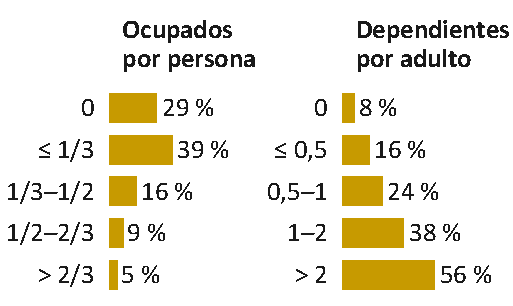
\includegraphics[width=\linewidth]{correlatos_pobreza}
    \column{0.34\textwidth}
      \footnotesize
      \textbf{Ingreso per cápita} $=$ cuántos trabajan $\times$ cuánto gana cada uno
      $\div$ cuántos comen.
      \begin{itemize}
        \item Más dependientes por adulto: pobreza de 8\,\% a 56\,\%.
        \item Jefe sin educación 40\,\%; con superior 8\,\%.
        \item Sin ocupados (29\,\%) es menos pobre que un tercio ocupado (39\,\%):
          pensiones y rentas.
      \end{itemize}
  \end{columns}
  \takeaway{Ninguna variable sola basta: la mejor regla de una variable da F1 de 0,473.}
  \fuente{Fuente: base de hogares de train (scripts/13\_figuras\_presentacion.R); views/tablas/leaderboard\_interno.csv.}
  \note{
    \textbf{Qué decir.} Partimos de la identidad del ingreso: cuántos trabajan, cuánto gana
    cada uno y entre cuántos se reparte. Los datos confirman cada pieza. Un patrón rompe el
    prior: los hogares sin ocupados no son los más pobres, porque muchos viven de pensiones
    o rentas. La relación no es lineal.\\[3pt]
    \textbf{Pregunta difícil: ¿basta con estas variables en un Logit?} No: un Logit con 5
    variables teóricas da F1 de 0,457, por debajo de la mejor regla de una variable
    (0,473). Con 48 variables construidas desde las personas sube a 0,718.
  }
\end{frame}

%% ============================================================
\section{Mejor modelo}
%% ============================================================
\begin{frame}{Confiamos en el holdout porque nunca se usó para decidir}
  \centering
  \begin{tikzpicture}[x=1cm,y=1cm,font=\scriptsize]
    \foreach \i in {0,...,4} {
      \fill[andeslight] (\i*1.9,0) rectangle ++(1.8,0.7);
      \pgfmathtruncatemacro{\k}{\i+1}
      \node at (\i*1.9+0.9,0.35) {fold \k};
    }
    \fill[andesaccent!35] (9.6,0) rectangle ++(2.6,0.7);
    \node at (10.9,0.35) {\textbf{holdout} 20\,\%};
    \draw[decorate,decoration={brace,amplitude=4pt}] (0,0.82) -- (9.4,0.82)
      node[midway,above=4pt] {80\,\% = 131.967 hogares: validación cruzada (CV) de 5 folds};
    \draw[decorate,decoration={brace,amplitude=4pt}] (9.6,0.82) -- (12.2,0.82)
      node[midway,above=4pt] {32.993 hogares};
    \node[draw=andesmid,rounded corners,fill=white,text width=6.2cm,align=left] (oof) at (4.7,-1.05)
      {Cada hogar recibe una predicción \textbf{fuera de fold (OOF)}, de un modelo que no lo
       vio. Con la OOF se eligen hiperparámetros, \textbf{umbral} y pesos de mezcla.};
    \node[draw=andesmid,rounded corners,fill=white,text width=3.2cm,align=left] (ho) at (10.9,-1.05)
      {Se mide una sola vez, con el umbral ya fijo.};
    \draw[-{Latex},andesgray] (4.7,-0.05) -- (oof.north);
    \draw[-{Latex},andesgray] (10.9,-0.05) -- (ho.north);
  \end{tikzpicture}
  \vspace{0.15cm}

  \raggedright\small
  \textbf{CV repetida:} al final repetimos la CV con 3 particiones nuevas (15 evaluaciones) y
  comparamos modelos con intervalos de confianza (IC: rango de valores compatibles con los datos) pareados por fold y por remuestra del holdout.
  \takeaway{La CV repetida reproduce la original casi al milésimo: 0,7752 frente a 0,7748.}
  \fuente{Fuente: views/tablas/resumen\_particion.csv; views/tablas/nivel7/etapa16\_fase1\_resumen.csv.}
  \note{
    \textbf{Qué decir.} Apartamos un 20\,\% al inicio y no lo tocamos. Todo lo que se
    elige (hiperparámetros, umbral, pesos) se elige con predicciones fuera de fold: cada
    hogar es predicho por un modelo que no lo vio. Al final repetimos la validación con
    tres particiones nuevas para medir cuánto ruido hay en una diferencia.\\[3pt]
    \textbf{Pregunta difícil: ¿no se sobreajustó el holdout tras muchas etapas?} Lo
    miramos muchas veces, aunque nunca para elegir parámetros. Por eso la comparación
    final usa la CV repetida en particiones nuevas, donde el orden de los candidatos se
    mantiene. Kaggle es la verificación externa.
  }
\end{frame}

\begin{frame}{Las variables aportaron 9 veces más F1 que el cambio de algoritmo}
  \begin{columns}[c]
    \column{0.66\textwidth}
      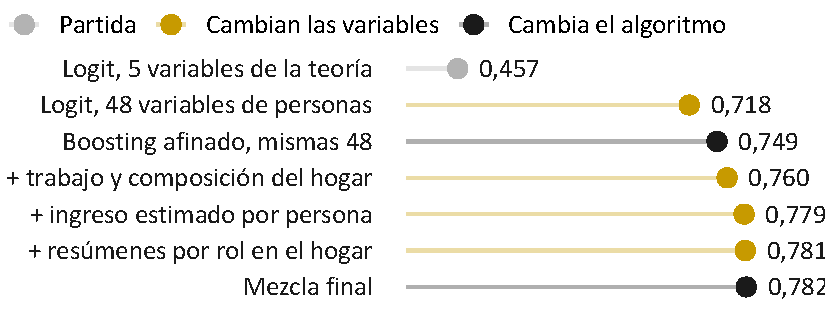
\includegraphics[width=\linewidth]{escalera_completa}
    \column{0.32\textwidth}
      \small
      \textbf{Suma de los saltos}
      \begin{itemize}
        \item \textcolor{andesaccent}{\textbf{Variables}}: $+0{,}292$.
        \item \textbf{Algoritmo}: $+0{,}032$.
      \end{itemize}
      El salto mayor (0,457 $\to$ 0,718) es el mismo Logit con variables construidas desde
      las personas.
  \end{columns}
  \takeaway{Rinde más entender el hogar que cambiar de algoritmo.}
  \fuente{F1 en holdout. Fuente: views/tablas/leaderboard\_interno.csv y nivel7/ (ablacion\_etapa1, resumen\_etapa2, etapa6\_ablacion, etapa7\_a, etapa18\_resumen).}
  \note{
    \textbf{Qué decir.} Cada punto es un paso de la escalera, medido en el mismo holdout.
    Los amarillos cambian las variables con el algoritmo fijo; los negros cambian el
    algoritmo con las variables fijas. Las variables suman 0,29 de F1; los algoritmos,
    0,03.\\[3pt]
    \textbf{Pregunta difícil: ¿la descomposición depende del orden?} Sí, es secuencial.
    Pero el contraste se sostiene en ambos sentidos: con 48 variables, pasar de Logit a
    XGBoost suma 0,029; con LightGBM fijo, pasar de 48 variables a la base final suma
    0,032; y otros algoritmos sobre la base final quedan entre 0,767 y 0,779.
  }
\end{frame}

\begin{frame}{El salto clave: predecir el ingreso de cada persona y sumarlo al hogar}
  \begin{columns}[c]
    \column{0.55\textwidth}
      \centering
      \begin{tikzpicture}[font=\scriptsize,
          caja/.style={draw=andesmid,rounded corners,fill=andeslight,text width=2.4cm,align=center,minimum height=0.8cm},
          clave/.style={caja,fill=andesyellow!45},
          flecha/.style={-{Latex},andesgray,thick}]
        \node[caja] (p) {Personas en train: ocupación, horas, cotización \textbf{+ su ingreso}};
        \node[clave,right=0.5cm of p] (m) {Modelo de ingreso por persona};
        \node[caja,below=0.45cm of m] (q) {Ingreso predicho de cada persona (también en test)};
        \node[caja,left=0.5cm of q] (h) {Suma del hogar $\div$ personas $\div$ línea};
        \node[clave,below=0.45cm of h] (c) {Clasificador del hogar};
        \draw[flecha] (p) -- (m);
        \draw[flecha] (m) -- (q);
        \draw[flecha] (q) -- (h);
        \draw[flecha] (h) -- (c);
      \end{tikzpicture}
    \column{0.43\textwidth}
      \tablachica
      \begin{tabular}{@{}lcc@{}}
        \toprule
        LightGBM con\ldots & F1 holdout & $\Delta$ \\
        \midrule
        sin auxiliares & 0,760 & \\
        + ingreso laboral & 0,771 & $+0{,}011$ \\
        + ingreso total & 0,776 & $+0{,}005$ \\
        + ingreso por fuente & 0,779 & $+0{,}003$ \\
        \bottomrule
      \end{tabular}
      \vspace{0.2cm}

      \footnotesize
      \textbf{OOF anidada:} el modelo de ingreso que alimenta a un hogar no vio ese hogar
      ni su fold de validación.
  \end{columns}
  \takeaway{El ingreso de train se usa como objetivo auxiliar, nunca como predictor.}
  \fuente{Fuente: views/tablas/nivel7/ablacion\_etapa1.csv, resumen\_etapa2.csv, etapa6\_ablacion.csv.}
  \note{
    \textbf{Qué decir.} En train sabemos cuánto gana cada persona. Entrenamos un modelo
    que predice ese ingreso con lo que el test sí trae. En test lo aplicamos, sumamos las
    predicciones del hogar y las dividimos por personas y por la línea. Solo el ingreso
    laboral predicho suma más de un punto de F1.\\[3pt]
    \textbf{Pregunta difícil: ¿no es fuga de información?} No, por construcción: cada
    hogar recibe la predicción de un modelo que no lo vio, y dentro de cada fold el
    auxiliar tampoco vio el fold de validación. Lo verifican tests automáticos. Con las
    1.306 variables observadas, un clasificador no distingue train de test (AUC 0,501);
    con los auxiliares sube a 0,713 porque en test se calculan con ajuste completo y en
    train fuera de fold.
  }
\end{frame}

\begin{frame}{El modelo decide con el ingreso predicho y con la vivienda}
  \begin{columns}[c]
    \column{0.60\textwidth}
      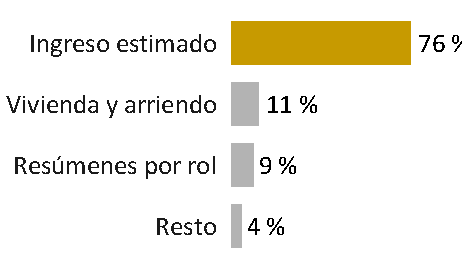
\includegraphics[width=\linewidth]{importancia_n7_a}
    \column{0.38\textwidth}
      \tablachica
      \begin{tabular}{@{}lrr@{}}
        \toprule
        Familia & Vars. & Ganancia \\
        \midrule
        Ingreso predicho & 17 & 75,6\,\% \\
        Vivienda y arriendo & 15 & 11,2\,\% \\
        Agregados por rol & 1.026 & 9,1\,\% \\
        Resto & 266 & 4,0\,\% \\
        \bottomrule
      \end{tabular}
      \vspace{0.15cm}

      \footnotesize
      En un boosting interpretable (EBM), la interacción más fuerte es arriendo por
      persona $\times$ vivienda propia pagada.
  \end{columns}
  \takeaway{El modelo reconstruye el ingreso y lo ajusta por el costo de la vivienda.}
  \fuente{Ganancia: reducción de la pérdida atribuida a cada variable en LightGBM (76\,\% de la mezcla). Fuente: views/tablas/nivel7/etapa7\_a\_importancia.csv, etapa15\_ebm\_importancia.csv.}
  \note{
    \textbf{Qué decir.} Tres cuartas partes de lo que aprende el modelo vienen de 17
    variables de ingreso predicho. Le sigue la vivienda: arriendo frente a la línea y
    tenencia. El arriendo revela capacidad de pago, y vivir en casa propia pagada es un
    ingreso implícito.\\[3pt]
    \textbf{Pregunta difícil: la ganancia favorece variables continuas.} Sí puede sesgar.
    Por eso lo contrastamos con un EBM, que mide el aporte medio al log-odds: también
    mandan el ingreso total predicho (0,57) y el arriendo por persona (0,50).
  }
\end{frame}

\begin{frame}{Los hiperparámetros importaron poco; el desbalance, nada}
  \begin{columns}[T]
    \column{0.52\textwidth}
      \tablachica
      \textbf{LightGBM}: 50 configuraciones (hipercubo latino), CV de 5 folds\\[3pt]
      \scriptsize
      \begin{tabular}{@{}lll@{}}
        \toprule
        Hiperparámetro & Valor & Lectura \\
        \midrule
        Rondas $\times$ tasa & 1.852 $\times$ 0,011 & aprende despacio \\
        Hojas por árbol & 31 & árboles pequeños \\
        Mínimo por hoja & 171 hogares & no memoriza \\
        Variables por corte & 82\,\% & algo de azar \\
        Hogares por árbol & 70\,\% & algo de azar \\
        \bottomrule
      \end{tabular}
    \column{0.44\textwidth}
      \footnotesize
      \begin{itemize}
        \item Reafinar con 75 intentos (Optuna) sobre las variables nuevas da el mismo F1:
          0,7759 frente a 0,7760.
        \item Promediar 5 semillas cambia el F1 en menos de 0,002.
        \item \textbf{Desbalance:} SMOTE, submuestreo y pesos de clase dan 0,745, 0,747 y
          0,744, frente a 0,746 sin balancear. Solo mueven el umbral óptimo (0,36 $\to$
          0,66 con pesos).
      \end{itemize}
  \end{columns}
  \takeaway{Elegir el umbral con OOF ya corrige el desbalance; rebalancear no agrega información.}
  \fuente{F1 en holdout. Fuente: views/tablas/leaderboard\_interno.csv; views/tablas/nivel7/resumen\_etapa2.csv.}
  \note{
    \textbf{Qué decir.} La configuración ganadora es conservadora: muchos árboles
    pequeños, aprendizaje lento y hojas de al menos 171 hogares. Buscar de nuevo con 75
    intentos no mejora. Rebalancear cambia la escala de las probabilidades, pero como el
    umbral se elige maximizando F1, el resultado es el mismo.\\[3pt]
    \textbf{Pregunta difícil: ¿por qué no tunear con el holdout?} Porque dejaría de ser
    una medida limpia. Todo el tuning usa F1 fuera de fold sobre el 80\,\%.
  }
\end{frame}

\begin{frame}{Dieciséis alternativas chocan con el mismo techo}
  \begin{columns}[c]
    \column{0.64\textwidth}
      \centering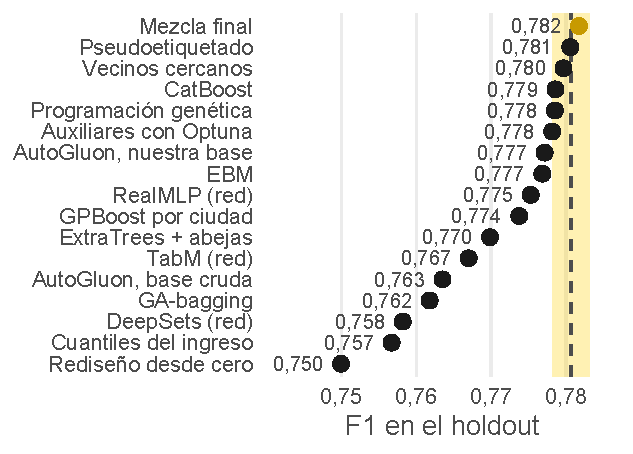
\includegraphics[height=5.3cm]{busqueda_techo}
    \column{0.34\textwidth}
      \footnotesize
      \textbf{Efecto mínimo detectable:} la mejora más pequeña que el holdout distingue del
      ruido es $\pm 0{,}0025$ (banda amarilla alrededor de LightGBM base, línea punteada).
      \begin{itemize}
        \item Ningún algoritmo nuevo supera a LightGBM.
        \item La mezcla final gana $+0{,}0007$ en CV repetida, IC 95\,\%
          [$+0{,}0002$; $+0{,}0012$]. Corrigiendo por la dependencia entre folds, el IC
          incluye cero.
      \end{itemize}
  \end{columns}
  \takeaway{Las mejoras posibles están por debajo de lo que los datos permiten detectar.}
  \fuente{F1 en holdout. Fuente: views/tablas/nivel7/ (etapa7\_b, etapa8 a etapa18); efecto mínimo de etapa16\_fase1\_resumen.csv.}
  \note{
    \textbf{Qué decir.} Probamos redes tabulares, AutoML, CatBoost, efectos aleatorios por
    ciudad, vecinos cercanos, programación genética de variables, pseudoetiquetado y un
    rediseño desde cero. Todos caen dentro o por debajo de la banda de ruido.\\[3pt]
    \textbf{Pregunta difícil: ¿por qué no quedarse con LightGBM solo?} Es nuestra
    recomendación práctica. La mezcla es la única que cumplió la regla fijada antes de la
    corrida (IC pareado sin cero en CV repetida y holdout no peor), pero gana milésimas y
    no sobrevive a la corrección por dependencia.
  }
\end{frame}

\begin{frame}{El techo está en los datos: sin el ingreso, un tercio de los pobres es indistinguible}
  \centering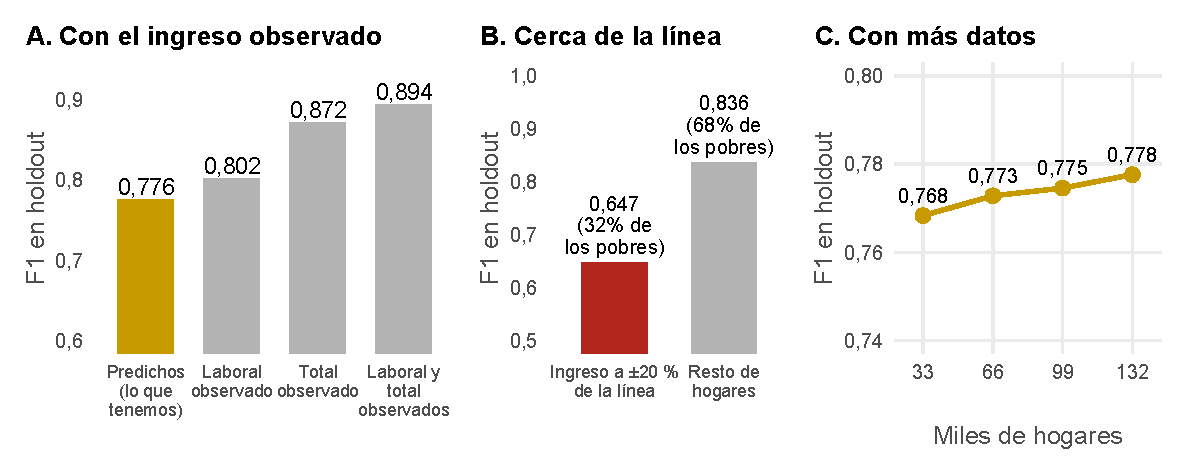
\includegraphics[height=3.85cm]{techo_tres_paneles}\par
  \raggedright\footnotesize
  \begin{columns}[T]
    \column{0.38\textwidth} \textbf{A.} Con el ingreso observado, el mismo modelo llegaría a 0,87--0,89.
    \column{0.30\textwidth} \textbf{B.} El 32\,\% de los pobres está a $\pm$\,20\,\% de la línea; ahí el F1 es 0,647.
    \column{0.28\textwidth} \textbf{C.} Cuadruplicar los datos sube el F1 solo 0,009.
  \end{columns}
  \takeaway{El límite viene sobre todo de la información que falta: el ingreso.}
  \fuente{Versión previa del modelo (LightGBM con auxiliares laboral y total), holdout. Fuente: views/tablas/nivel7/techo\_oraculo.csv, techo\_bandas.csv, techo\_curva\_aprendizaje.csv.}
  \note{
    \textbf{Qué decir.} Tres pruebas de que el techo es de información. Con el ingreso
    real, el F1 subiría a casi 0,9: el error que queda es el de predecir el ingreso. Ese
    error pesa cerca de la línea, donde está un tercio de los pobres y el F1 cae a 0,65. Y
    más datos casi no ayudan: la curva de aprendizaje es plana.\\[3pt]
    \textbf{Pregunta difícil: ¿por qué el oráculo no da F1 = 1?} Porque el ingreso de las
    personas no incluye el arriendo imputado a propietarios, que sí entra en el ingreso
    del hogar que define la pobreza.
  }
\end{frame}

%% ============================================================
\section{Implicaciones de política}
%% ============================================================
\begin{frame}{Excluimos al 18\,\% de los pobres, sobre todo a los más cercanos a la línea}
  \begin{columns}[c]
    \column{0.58\textwidth}
      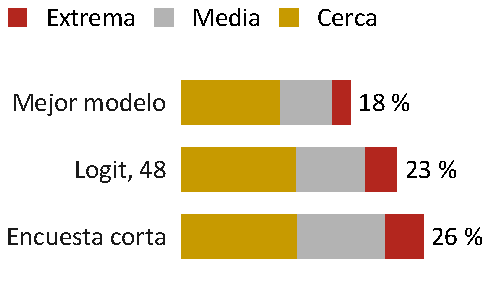
\includegraphics[width=\linewidth]{excluidos_por_modelo}
    \column{0.40\textwidth}
      \footnotesize
      \begin{itemize}
        \item \textbf{Subcobertura} 18,2\,\% (1.201 de 6.605 pobres). Brecha media de los
          excluidos: 0,22, frente a 0,37 del pobre promedio.
        \item \textbf{Filtración} 25,1\,\%, pero los no pobres incluidos están cerca: distancia
          media a la línea 0,51 (el no pobre promedio: 2,83).
        \item Más subcobertura en hogares de 1 y 2 personas (34\,\% y 28\,\%), Manizales
          (36\,\%) y Pereira (29\,\%).
      \end{itemize}
  \end{columns}
  \takeaway{Ponderando cada error por su distancia a la línea, la subcobertura baja a 11,2\,\% y la filtración a 1,2\,\%.}
  \fuente{Holdout, umbral 0,36; brecha $=1-$ingreso/línea. Mezcla sin el modelo limpio (95\,\% del peso del final). Fuente: views/tablas/nivel7/etapa15\_pesos\_bienestar.csv, etapa15\_errores\_subgrupo.csv.}
  \note{
    \textbf{Qué decir.} El F1 trata igual todos los errores, pero no cuestan lo mismo. El
    59\,\% de los pobres que dejamos fuera tiene ingreso de al menos 0,8 veces la línea, y
    los no pobres incluidos también están cerca. Ponderando cada error por su distancia a
    la línea, la subcobertura baja de 18 a 11\,\%.\\[3pt]
    \textbf{Pregunta difícil: ¿hay sesgo contra hogares pequeños?} Sí hay más
    subcobertura en hogares de 1 y 2 personas: su ingreso depende de una sola persona y es
    más difícil de predecir. Una agencia podría fijar un umbral más bajo para ese grupo.
  }
\end{frame}

\begin{frame}{Una encuesta corta excluye a más pobres, y a más pobres extremos}
  \begin{columns}[c]
    \column{0.52\textwidth}
      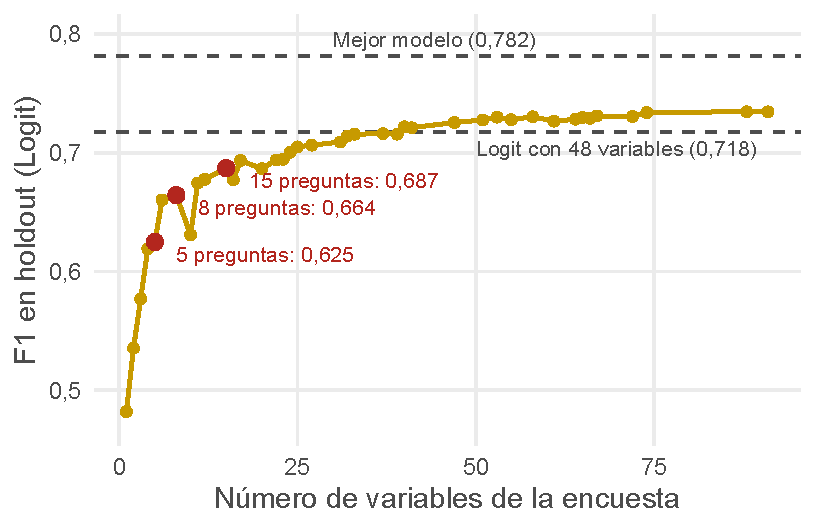
\includegraphics[width=\linewidth]{frontera_encuesta}
    \column{0.46\textwidth}
      \footnotesize
      \textbf{Intuición.} El mejor modelo necesita el módulo laboral de cada persona: es
      largo y autorreportado.
      \begin{itemize}
        \item Logit con las 8 mejores preguntas (ocupados, horas, cotizantes, quién quiere
          más horas, arriendo pagado y recibido, dormitorios): F1 0,664 frente a 0,782.
        \item Subcobertura 26,0\,\% y filtración 39,8\,\%.
        \item El 16\,\% de sus excluidos está en pobreza extrema (11\,\% con el mejor modelo).
      \end{itemize}
  \end{columns}
  \takeaway{Acortar la encuesta ahorra costo, pero corre la exclusión hacia los más pobres.}
  \fuente{Preguntas elegidas con NSGA-II (algoritmo genético con dos objetivos: F1 y número de preguntas). Fuente: views/tablas/nivel7/frontera\_encuesta\_corta.csv, etapa15\_pesos\_bienestar.csv.}
  \note{
    \textbf{Qué decir.} Buscamos el mejor conjunto de preguntas para cada tamaño de
    encuesta. Con 8 preguntas el F1 baja de 0,78 a 0,66, y lo más grave es a quiénes
    excluye: la exclusión se corre hacia la pobreza extrema.\\[3pt]
    \textbf{Pregunta difícil: ¿no pueden usar el modelo de ingreso en la encuesta corta?}
    No sin el módulo laboral: el auxiliar se alimenta de la ocupación, horas y cotización
    de cada persona. Por eso la frontera se construyó sin auxiliares.
  }
\end{frame}

\begin{frame}{El umbral es una decisión de política: la agencia puede comprar cobertura}
  \begin{columns}[c]
    \column{0.50\textwidth}
      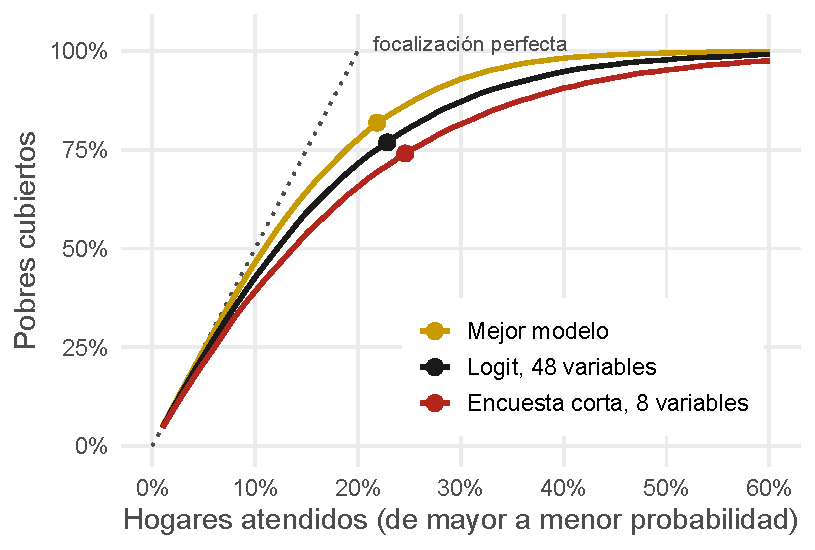
\includegraphics[width=\linewidth]{curva_cobertura_slides}
    \column{0.48\textwidth}
      \footnotesize
      \textbf{El umbral que maximiza F1 supone que ambos errores cuestan igual.}
      \begin{itemize}
        \item Atendiendo al 25\,\% de los hogares se cubre al 86,8\,\% de los pobres; al
          30\,\%, al 92,9\,\%.
        \item Bajar el umbral de 0,38 a 0,21 reduce la subcobertura de 19,3\,\% a 9,7\,\%;
          la filtración sube de 26,5\,\% a 36,2\,\% y el F1 apenas cae (0,769 a 0,747).
        \item La encuesta corta necesita atender al 40\,\% para cubrir al 90,6\,\%.
      \end{itemize}
  \end{columns}
  \takeaway{Si excluir a un pobre cuesta más que incluir a un no pobre, conviene bajar el umbral.}
  \fuente{Puntos: umbral elegido con OOF. Fuente: views/tablas/nivel7/etapa15\_curva\_cobertura.csv (holdout); views/tablas/escenarios\_politica\_n7.csv (OOF de la versión previa con auxiliares laboral y total).}
  \note{
    \textbf{Qué decir.} El F1 pondera igual los dos errores. Una agencia que valora más no
    dejar pobres por fuera puede bajar el umbral: la subcobertura se reduce a la mitad
    con 10 puntos más de filtración. Como los filtrados están cerca de la línea, ese costo
    es bajo en bienestar.\\[3pt]
    \textbf{Pregunta difícil: ¿qué umbral recomiendan?} Depende del costo relativo que
    fije la política. Con costos iguales, el del F1; si excluir cuesta el doble, uno más
    bajo. Es una decisión normativa, no estadística.
  }
\end{frame}

\begin{frame}{Recomendación a la agencia: medir bien el trabajo de cada persona}
  \small
  \begin{enumerate}
    \item \textbf{Con módulo laboral por persona:} modelo de ingreso por persona +
      LightGBM. Un LightGBM solo rinde igual que la mezcla y es más fácil de mantener.
    \item \textbf{Umbral según el costo de excluir, no según F1:} con un umbral menor la
      subcobertura baja de 19\,\% a 10\,\%, a cambio de filtración cerca de la línea.
    \item \textbf{Con presupuesto solo para encuesta corta:} usarla como filtro amplio
      (atender al 40\,\% cubre al 91\,\% de los pobres) y verificar con la encuesta larga a
      quienes quedan cerca del umbral.
    \item \textbf{Vigilar los grupos con más subcobertura:} hogares de 1--2 personas,
      Manizales y Pereira.
    \item \textbf{No esperar más de más modelos:} el techo es de información.
  \end{enumerate}
  \takeaway{El valor está en medir el ingreso; el algoritmo es secundario.}
  \note{
    \textbf{Qué decir.} Cinco recomendaciones que se siguen de la evidencia: el modelo
    sirve si se puede preguntar por el trabajo de cada persona; el umbral es una decisión
    de política; una encuesta corta funciona como primer filtro si se acepta más
    filtración; hay grupos que vigilar; y el límite es de información.\\[3pt]
    \textbf{Pregunta difícil: ¿son verificables las variables clave?} En parte. Tenencia
    y arriendo se pueden observar en una visita; horas e ingresos son autorreportados.
    Por eso recomendamos verificar en campo a los hogares cercanos al umbral, donde el
    modelo es menos confiable.
  }
\end{frame}

%% ============================================================
%% Apéndice
%% ============================================================
\appendix
\diapositivaglosario

\begin{frame}{Apéndice: auditoría de los datos, sin fuga ni errores de construcción}
  \small
  \begin{columns}[T]
    \column{0.48\textwidth}
      \textbf{Construcción}
      \begin{itemize}
        \item 0 personas sin hogar; 0 hogares sin jefe o con varios jefes.
        \item Pobre $=$ (ingreso per cápita $<$ línea) en los 164.960 hogares.
        \item Ids de train y test sin intersección.
      \end{itemize}
    \column{0.48\textwidth}
      \textbf{Fuga y cambio de distribución}
      \begin{itemize}
        \item Validación adversarial (¿se distingue train de test?): AUC 0,501 con las
          variables observadas; 0,713 con los auxiliares, por su ajuste completo en test.
        \item Reponderar por esa diferencia no cambia el F1 (IC con cero).
      \end{itemize}
  \end{columns}
  \fuente{Fuente: views/tablas/nivel7/forense\_resumen.csv, forense\_adversarial.csv, forense\_experimentos.csv.}
  \note{Respaldo para preguntas sobre fuga o cambio de distribución.}
\end{frame}

\begin{frame}{Apéndice: en CV repetida ninguna alternativa mejora de forma detectable}
  \centering\scriptsize
  \begin{tabular}{@{}lccc@{}}
    \toprule
    Candidato & F1 CV repetida (EE) & $\Delta$ vs.\ LightGBM [IC 95\,\%] & F1 holdout [IC 95\,\%] \\
    \midrule
    LightGBM base & 0,7752 (0,0008) & & 0,7806 [0,7731; 0,7885] \\
    + redes (mezcla sin limpio) & 0,7758 (0,0008) & $+0{,}0006$ [$-0{,}0001$; $+0{,}0013$] & 0,7820 [0,7743; 0,7897] \\
    \textbf{+ redes + limpio (final)} & \textbf{0,7759 (0,0008)} & $+0{,}0007$ [$+0{,}0002$; $+0{,}0012$] & 0,7817 [0,7742; 0,7894] \\
    CatBoost & 0,7722 (0,0007) & $-0{,}0030$ [$-0{,}0042$; $-0{,}0018$] & 0,7786 [0,7707; 0,7864] \\
    Base con códigos corregidos & 0,7754 (0,0008) & $+0{,}0002$ [$-0{,}0002$; $+0{,}0005$] & 0,7797 [0,7720; 0,7875] \\
    Rediseño desde cero & 0,7478 (0,0008) & $-0{,}0274$ [$-0{,}0289$; $-0{,}0260$] & 0,7499 [0,7420; 0,7581] \\
    \bottomrule
  \end{tabular}
  \fuente{IC pareados ingenuos (15 pares). Con la corrección de Nadeau y Bengio el IC del modelo final es [$-0{,}0004$; $+0{,}0017$]. Fuente: views/tablas/nivel7/etapa16\_fase1\_resumen.csv, etapa18\_resumen.csv.}
  \note{Respaldo: la única diferencia cuyo IC ingenuo excluye cero es la del modelo final, y por milésimas.}
\end{frame}

\begin{frame}{Apéndice: un rediseño desde cero llega a 0,750; le falta el ingreso por persona}
  \small
  \begin{itemize}
    \item Rehicimos el pipeline sin mirar el trabajo previo: 74 variables de hogar a partir
      del diccionario del DANE, con los códigos de ``no sabe'' como faltantes.
    \item Una variante con el ingreso del hogar como objetivo auxiliar (anidado) no mejora.
    \item F1 en CV repetida 0,748 y holdout 0,750, frente a 0,775 y 0,781 de LightGBM base;
      correlación de sus predicciones con LightGBM: 0,94.
    \item Lo que separa a los dos pipelines es predecir el ingreso de cada persona, no el
      del hogar.
  \end{itemize}
  \fuente{Fuente: limpio/resultados/; views/tablas/nivel7/etapa18\_resumen.csv.}
  \note{Respaldo: el rediseño confirma que el auxiliar a nivel persona es la pieza clave.}
\end{frame}

\end{document}
"
%% ============================================================
\documentclass[aspectratio=169,11pt]{beamer}
%% Preamble: packages and theme. Keep design changes in beamerthemeUniandes.sty
\usepackage[utf8]{inputenc}
\usepackage[T1]{fontenc}
\usepackage[spanish,es-nodecimaldot,es-noshorthands]{babel}
\usepackage{amsmath,amssymb}
\usepackage{graphicx}
\usepackage{booktabs}
\usepackage[round]{natbib}
\usetheme{Uniandes}

%% ---- Agregados para el Problem Set 2 (no cambian el diseño) ----
% Algunas instalaciones de MiKTeX no registran el mapa de Source Sans; se carga aquí.
\pdfmapfile{+SourceSansThree.map}
\usepackage{array}
\usepackage{xspace}
\usetikzlibrary{positioning,arrows.meta,decorations.pathreplacing}
\graphicspath{{../figuras/}{../../../views/figuras/}{../../../views/figuras/nivel7/}}

% Notas del presentador: el PDF de entrega no las muestra; la versión *_notas
% se compila con \def\connotas{} antes del documento y las intercala.
\ifdefined\connotas
  \setbeameroption{show notes}
\else
  \setbeameroption{hide notes}
\fi
\setbeamerfont{note page}{size=\small}
\setbeamertemplate{note page}{%
  \vspace{0.3cm}\insertslideintonotes{0.25}\par\vspace{0.2cm}
  \begin{minipage}{0.95\textwidth}\insertnote\end{minipage}}

% F1 público de Kaggle del mejor modelo (n18), tal como lo muestra la Overview.
\def\kagglepublico{0,78}

% Tabla pequeña con letra reducida
\newcommand{\tablachica}{\footnotesize\renewcommand{\arraystretch}{1.12}}
% Fuente de una figura o tabla, al pie
\newcommand{\fuente}[1]{\par\vspace{2pt}{\tiny\color{andesgray}#1\par}}
% Títulos sin cortar palabras con guion: se hace dentro de la plantilla del título
% (beamerthemeUniandes.sty), porque el minipage del título reinicia la alineación.
% Cajas de los diagramas sin guiones
\tikzset{every node/.append style={execute at begin node={\hyphenpenalty=10000\exhyphenpenalty=10000}}}

%% ============================================================
%%  Piezas comunes a los dos decks: Best Model Overview y glosario
%% ============================================================

% ---- Best Model Overview (diapositiva obligatoria, primera de cada deck) ----
\newcommand{\diapositivaoverview}{%
\begin{frame}{Best Model Overview}
  {Ingreso predicho por persona + LightGBM \;|\; Equipo 06, MECA 4107}
  \vspace{-0.1cm}
  \begin{columns}[T]
    \column{0.37\textwidth}\centering \keyfig{\kagglepublico}{F1 público en Kaggle}
    \column{0.30\textwidth}\centering \keyfig{0,782}{F1 en holdout, IC 95\,\% [0,774; 0,789]}
    \column{0.30\textwidth}\centering \keyfig{0,776}{F1 en CV repetida (15 evaluaciones)}
  \end{columns}
  \vspace{0.15cm}
  \footnotesize
  \begin{columns}[T]
    \column{0.49\textwidth}
      \textbf{Especificación}
      \begin{itemize}
        \item \textbf{Variable clave:} el ingreso de cada persona, predicho con lo que el test
          sí trae y sumado al hogar (1.324 variables en total).
        \item \textbf{Algoritmo:} LightGBM (76\,\%) mezclado con dos redes (19\,\%) y un
          rediseño desde cero (5\,\%); pesos elegidos fuera de muestra.
        \item \textbf{Regla:} pobre si $P(\text{pobre}) \geq 0{,}36$.
      \end{itemize}
    \column{0.49\textwidth}
      \textbf{Mensajes}
      \begin{enumerate}
        \item Las variables aportaron \textbf{9 veces más} F1 que los algoritmos.
        \item El techo (${\approx}\,0{,}78$) viene sobre todo de la información que falta.
        \item Excluye al 18\,\% de los pobres, casi todos cerca de la línea.
      \end{enumerate}
  \end{columns}
  \fuente{F1: media armónica de precisión y recall de la clase pobre. Holdout: 20\,\% del train nunca usado para decidir. Fuente: views/tablas/nivel7/etapa18\_resumen.csv.}
  \note{
    \textbf{Qué decir (1 min).} Nuestro mejor modelo clasifica hogares pobres con F1 de
    0,782 en datos que nunca usamos para decidir. La pieza clave no es el algoritmo sino
    una variable: predecimos cuánto gana cada persona con lo que el test sí trae
    (ocupación, horas, cotización) y lo sumamos al hogar. Tres mensajes: las variables
    pesan 9 veces más que el algoritmo, hay un techo que viene de los datos y los errores
    se concentran cerca de la línea.\\[3pt]
    \textbf{Pregunta difícil: ¿por qué una mezcla y no un solo modelo?} La mezcla gana
    +0,0007 en CV repetida frente a LightGBM solo. El IC ingenuo [+0,0002; +0,0012] excluye
    cero; el corregido por dependencia entre folds no. Es una mejora marginal: en la
    práctica LightGBM solo rinde igual.
  }
\end{frame}}

% ---- Glosario (apéndice de ambos decks, dos diapositivas) ----
\newcommand{\filaglosario}[2]{\textbf{#1} & #2 \\}
\newcommand{\diapositivaglosario}{%
\begin{frame}{Glosario (1/2): métricas y errores}
  \footnotesize\renewcommand{\arraystretch}{1.25}
  \begin{tabular}{@{}p{0.2\textwidth}p{0.76\textwidth}@{}}
    \toprule
    \filaglosario{Precisión}{De los hogares que el programa atiende, qué parte es pobre. $1-$precisión $=$ \textbf{filtración}: no pobres que reciben el beneficio.}
    \filaglosario{Recall}{De los hogares pobres, qué parte atiende el programa. $1-$recall $=$ \textbf{subcobertura}: pobres excluidos.}
    \filaglosario{F1}{Media armónica de precisión y recall: solo es alta si ambas lo son. No premia a los no pobres bien clasificados.}
    \filaglosario{Umbral}{Probabilidad a partir de la cual un hogar se clasifica como pobre. Bajarlo cubre más pobres a cambio de más filtración.}
    \filaglosario{IC 95\,\%}{Rango de valores compatibles con los datos. Si el IC de una diferencia incluye cero, no podemos afirmar que haya mejora.}
    \filaglosario{Efecto mínimo detectable}{La mejora más pequeña que el diseño detectaría con probabilidad 0,8.}
    \bottomrule
  \end{tabular}
  \note{Glosario de apoyo; se muestra solo si lo preguntan.}
\end{frame}
\begin{frame}{Glosario (2/2): validación y variables}
  \footnotesize\renewcommand{\arraystretch}{1.25}
  \begin{tabular}{@{}p{0.2\textwidth}p{0.76\textwidth}@{}}
    \toprule
    \filaglosario{Holdout}{20\,\% del train (32.993 hogares) apartado al inicio; solo se usa para medir, nunca para decidir.}
    \filaglosario{Validación cruzada}{El 80\,\% restante se parte en 5 bloques (folds): se entrena con 4 y se evalúa en el quinto, rotando.}
    \filaglosario{Fuera de fold (OOF)}{La predicción de cada hogar hecha por un modelo que no lo vio. Con ella se eligen umbral, pesos e hiperparámetros.}
    \filaglosario{CV repetida}{La validación cruzada repetida con 3 particiones nuevas: 15 evaluaciones para medir la variabilidad.}
    \filaglosario{Auxiliar de ingreso}{Modelo que predice el ingreso de cada persona con variables que el test sí trae; sumado al hogar, entra como variable.}
    \filaglosario{OOF anidada}{El auxiliar que alimenta a un hogar no vio ese hogar ni su fold de validación: así no se filtra la respuesta.}
    \bottomrule
  \end{tabular}
  \note{Glosario de apoyo; se muestra solo si lo preguntan.}
\end{frame}}


\title[Predicting Poverty: Best Model Deep Dive]{Predicting Poverty: Best Model Deep Dive}
\author[Labastidas y Garcia | Equipo 06]{Esteban David Labastidas Martínez \and Neislen Stiven Garcia Silva}
\institute{Facultad de Economía\\ Universidad de los Andes}
\date[Oct 2026]{Bogotá, octubre de 2026}

\begin{document}
\andessectionslidesfalse

%% 1. Best Model Overview (obligatoria)
\diapositivaoverview

%% ============================================================
\section{Datos}
%% ============================================================
\begin{frame}{El test no trae ingresos: hay que inferir la pobreza sin ver su definición}
  \begin{columns}[T]
    \column{0.62\textwidth}
      \small
      \textbf{Intuición.} Un hogar es pobre si su ingreso per cápita está bajo la línea de
      pobreza de su ciudad y mes. El test no trae ningún ingreso.
      \begin{itemize}
        \item 79 variables solo existen en train, entre ellas todos los ingresos.
        \item Pobre $\Leftrightarrow$ ingreso per cápita $<$ línea, sin excepciones.
        \item Bogotá está en train pero no en test.
      \end{itemize}
      \textbf{Métrica.} ``Nadie es pobre'' acierta en el 80\,\% de los hogares, pero tiene
      F1 $=0$. El F1 combina \textbf{filtración} (no pobres atendidos) y
      \textbf{subcobertura} (pobres excluidos).
    \column{0.34\textwidth}
      \centering
      \keyfig{164.960}{hogares en train}\\[0.02cm]
      \keyfig{66.168}{hogares en test}\\[0.02cm]
      \keyfig{20,0\,\%}{hogares pobres}
  \end{columns}
  \takeaway{El problema es reconstruir el ingreso con lo que sí se observa.}
  \fuente{Fuente: views/tablas/nivel7/forense\_resumen.csv; views/tablas/desbalance\_clases.csv.}
  \note{
    \textbf{Qué decir.} La definición de pobreza es mecánica: ingreso per cápita contra la
    línea. El reto es que el test no trae ingresos, así que hay que inferirlos de lo
    observable. La clase pobre es una de cada cinco; por eso no usamos accuracy sino F1, que
    castiga tanto dejar pobres por fuera (subcobertura) como incluir no pobres
    (filtración).\\[3pt]
    \textbf{Pregunta difícil: ¿por qué no predecir el ingreso y aplicar la línea?} El
    enunciado pide clasificación. Usamos el ingreso solo como objetivo auxiliar por
    persona, nunca como predictor; el clasificador final predice la etiqueta.
  }
\end{frame}

\begin{frame}{La teoría acierta: trabajo, dependencia, educación y vivienda predicen la pobreza}
  \begin{columns}[c]
    \column{0.64\textwidth}
      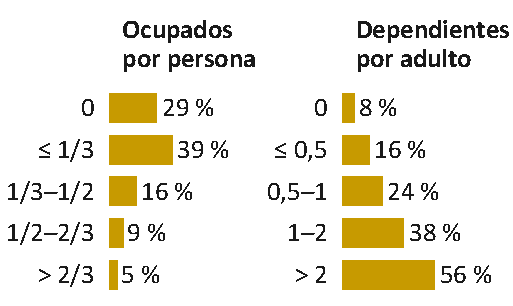
\includegraphics[width=\linewidth]{correlatos_pobreza}
    \column{0.34\textwidth}
      \footnotesize
      \textbf{Ingreso per cápita} $=$ cuántos trabajan $\times$ cuánto gana cada uno
      $\div$ cuántos comen.
      \begin{itemize}
        \item Más dependientes por adulto: pobreza de 8\,\% a 56\,\%.
        \item Jefe sin educación 40\,\%; con superior 8\,\%.
        \item Sin ocupados (29\,\%) es menos pobre que un tercio ocupado (39\,\%):
          pensiones y rentas.
      \end{itemize}
  \end{columns}
  \takeaway{Ninguna variable sola basta: la mejor regla de una variable da F1 de 0,473.}
  \fuente{Fuente: base de hogares de train (scripts/13\_figuras\_presentacion.R); views/tablas/leaderboard\_interno.csv.}
  \note{
    \textbf{Qué decir.} Partimos de la identidad del ingreso: cuántos trabajan, cuánto gana
    cada uno y entre cuántos se reparte. Los datos confirman cada pieza. Un patrón rompe el
    prior: los hogares sin ocupados no son los más pobres, porque muchos viven de pensiones
    o rentas. La relación no es lineal.\\[3pt]
    \textbf{Pregunta difícil: ¿basta con estas variables en un Logit?} No: un Logit con 5
    variables teóricas da F1 de 0,457, por debajo de la mejor regla de una variable
    (0,473). Con 48 variables construidas desde las personas sube a 0,718.
  }
\end{frame}

%% ============================================================
\section{Mejor modelo}
%% ============================================================
\begin{frame}{Confiamos en el holdout porque nunca se usó para decidir}
  \centering
  \begin{tikzpicture}[x=1cm,y=1cm,font=\scriptsize]
    \foreach \i in {0,...,4} {
      \fill[andeslight] (\i*1.9,0) rectangle ++(1.8,0.7);
      \pgfmathtruncatemacro{\k}{\i+1}
      \node at (\i*1.9+0.9,0.35) {fold \k};
    }
    \fill[andesaccent!35] (9.6,0) rectangle ++(2.6,0.7);
    \node at (10.9,0.35) {\textbf{holdout} 20\,\%};
    \draw[decorate,decoration={brace,amplitude=4pt}] (0,0.82) -- (9.4,0.82)
      node[midway,above=4pt] {80\,\% = 131.967 hogares: validación cruzada (CV) de 5 folds};
    \draw[decorate,decoration={brace,amplitude=4pt}] (9.6,0.82) -- (12.2,0.82)
      node[midway,above=4pt] {32.993 hogares};
    \node[draw=andesmid,rounded corners,fill=white,text width=6.2cm,align=left] (oof) at (4.7,-1.05)
      {Cada hogar recibe una predicción \textbf{fuera de fold (OOF)}, de un modelo que no lo
       vio. Con la OOF se eligen hiperparámetros, \textbf{umbral} y pesos de mezcla.};
    \node[draw=andesmid,rounded corners,fill=white,text width=3.2cm,align=left] (ho) at (10.9,-1.05)
      {Se mide una sola vez, con el umbral ya fijo.};
    \draw[-{Latex},andesgray] (4.7,-0.05) -- (oof.north);
    \draw[-{Latex},andesgray] (10.9,-0.05) -- (ho.north);
  \end{tikzpicture}
  \vspace{0.15cm}

  \raggedright\small
  \textbf{CV repetida:} al final repetimos la CV con 3 particiones nuevas (15 evaluaciones) y
  comparamos modelos con intervalos de confianza (IC: rango de valores compatibles con los datos) pareados por fold y por remuestra del holdout.
  \takeaway{La CV repetida reproduce la original casi al milésimo: 0,7752 frente a 0,7748.}
  \fuente{Fuente: views/tablas/resumen\_particion.csv; views/tablas/nivel7/etapa16\_fase1\_resumen.csv.}
  \note{
    \textbf{Qué decir.} Apartamos un 20\,\% al inicio y no lo tocamos. Todo lo que se
    elige (hiperparámetros, umbral, pesos) se elige con predicciones fuera de fold: cada
    hogar es predicho por un modelo que no lo vio. Al final repetimos la validación con
    tres particiones nuevas para medir cuánto ruido hay en una diferencia.\\[3pt]
    \textbf{Pregunta difícil: ¿no se sobreajustó el holdout tras muchas etapas?} Lo
    miramos muchas veces, aunque nunca para elegir parámetros. Por eso la comparación
    final usa la CV repetida en particiones nuevas, donde el orden de los candidatos se
    mantiene. Kaggle es la verificación externa.
  }
\end{frame}

\begin{frame}{Las variables aportaron 9 veces más F1 que el cambio de algoritmo}
  \begin{columns}[c]
    \column{0.66\textwidth}
      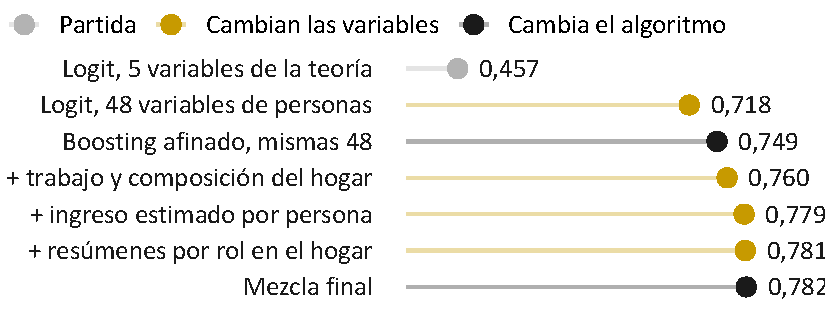
\includegraphics[width=\linewidth]{escalera_completa}
    \column{0.32\textwidth}
      \small
      \textbf{Suma de los saltos}
      \begin{itemize}
        \item \textcolor{andesaccent}{\textbf{Variables}}: $+0{,}292$.
        \item \textbf{Algoritmo}: $+0{,}032$.
      \end{itemize}
      El salto mayor (0,457 $\to$ 0,718) es el mismo Logit con variables construidas desde
      las personas.
  \end{columns}
  \takeaway{Rinde más entender el hogar que cambiar de algoritmo.}
  \fuente{F1 en holdout. Fuente: views/tablas/leaderboard\_interno.csv y nivel7/ (ablacion\_etapa1, resumen\_etapa2, etapa6\_ablacion, etapa7\_a, etapa18\_resumen).}
  \note{
    \textbf{Qué decir.} Cada punto es un paso de la escalera, medido en el mismo holdout.
    Los amarillos cambian las variables con el algoritmo fijo; los negros cambian el
    algoritmo con las variables fijas. Las variables suman 0,29 de F1; los algoritmos,
    0,03.\\[3pt]
    \textbf{Pregunta difícil: ¿la descomposición depende del orden?} Sí, es secuencial.
    Pero el contraste se sostiene en ambos sentidos: con 48 variables, pasar de Logit a
    XGBoost suma 0,029; con LightGBM fijo, pasar de 48 variables a la base final suma
    0,032; y otros algoritmos sobre la base final quedan entre 0,767 y 0,779.
  }
\end{frame}

\begin{frame}{El salto clave: predecir el ingreso de cada persona y sumarlo al hogar}
  \begin{columns}[c]
    \column{0.55\textwidth}
      \centering
      \begin{tikzpicture}[font=\scriptsize,
          caja/.style={draw=andesmid,rounded corners,fill=andeslight,text width=2.4cm,align=center,minimum height=0.8cm},
          clave/.style={caja,fill=andesyellow!45},
          flecha/.style={-{Latex},andesgray,thick}]
        \node[caja] (p) {Personas en train: ocupación, horas, cotización \textbf{+ su ingreso}};
        \node[clave,right=0.5cm of p] (m) {Modelo de ingreso por persona};
        \node[caja,below=0.45cm of m] (q) {Ingreso predicho de cada persona (también en test)};
        \node[caja,left=0.5cm of q] (h) {Suma del hogar $\div$ personas $\div$ línea};
        \node[clave,below=0.45cm of h] (c) {Clasificador del hogar};
        \draw[flecha] (p) -- (m);
        \draw[flecha] (m) -- (q);
        \draw[flecha] (q) -- (h);
        \draw[flecha] (h) -- (c);
      \end{tikzpicture}
    \column{0.43\textwidth}
      \tablachica
      \begin{tabular}{@{}lcc@{}}
        \toprule
        LightGBM con\ldots & F1 holdout & $\Delta$ \\
        \midrule
        sin auxiliares & 0,760 & \\
        + ingreso laboral & 0,771 & $+0{,}011$ \\
        + ingreso total & 0,776 & $+0{,}005$ \\
        + ingreso por fuente & 0,779 & $+0{,}003$ \\
        \bottomrule
      \end{tabular}
      \vspace{0.2cm}

      \footnotesize
      \textbf{OOF anidada:} el modelo de ingreso que alimenta a un hogar no vio ese hogar
      ni su fold de validación.
  \end{columns}
  \takeaway{El ingreso de train se usa como objetivo auxiliar, nunca como predictor.}
  \fuente{Fuente: views/tablas/nivel7/ablacion\_etapa1.csv, resumen\_etapa2.csv, etapa6\_ablacion.csv.}
  \note{
    \textbf{Qué decir.} En train sabemos cuánto gana cada persona. Entrenamos un modelo
    que predice ese ingreso con lo que el test sí trae. En test lo aplicamos, sumamos las
    predicciones del hogar y las dividimos por personas y por la línea. Solo el ingreso
    laboral predicho suma más de un punto de F1.\\[3pt]
    \textbf{Pregunta difícil: ¿no es fuga de información?} No, por construcción: cada
    hogar recibe la predicción de un modelo que no lo vio, y dentro de cada fold el
    auxiliar tampoco vio el fold de validación. Lo verifican tests automáticos. Con las
    1.306 variables observadas, un clasificador no distingue train de test (AUC 0,501);
    con los auxiliares sube a 0,713 porque en test se calculan con ajuste completo y en
    train fuera de fold.
  }
\end{frame}

\begin{frame}{El modelo decide con el ingreso predicho y con la vivienda}
  \begin{columns}[c]
    \column{0.60\textwidth}
      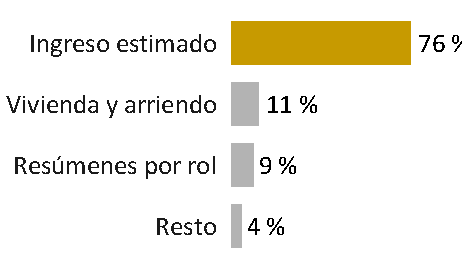
\includegraphics[width=\linewidth]{importancia_n7_a}
    \column{0.38\textwidth}
      \tablachica
      \begin{tabular}{@{}lrr@{}}
        \toprule
        Familia & Vars. & Ganancia \\
        \midrule
        Ingreso predicho & 17 & 75,6\,\% \\
        Vivienda y arriendo & 15 & 11,2\,\% \\
        Agregados por rol & 1.026 & 9,1\,\% \\
        Resto & 266 & 4,0\,\% \\
        \bottomrule
      \end{tabular}
      \vspace{0.15cm}

      \footnotesize
      En un boosting interpretable (EBM), la interacción más fuerte es arriendo por
      persona $\times$ vivienda propia pagada.
  \end{columns}
  \takeaway{El modelo reconstruye el ingreso y lo ajusta por el costo de la vivienda.}
  \fuente{Ganancia: reducción de la pérdida atribuida a cada variable en LightGBM (76\,\% de la mezcla). Fuente: views/tablas/nivel7/etapa7\_a\_importancia.csv, etapa15\_ebm\_importancia.csv.}
  \note{
    \textbf{Qué decir.} Tres cuartas partes de lo que aprende el modelo vienen de 17
    variables de ingreso predicho. Le sigue la vivienda: arriendo frente a la línea y
    tenencia. El arriendo revela capacidad de pago, y vivir en casa propia pagada es un
    ingreso implícito.\\[3pt]
    \textbf{Pregunta difícil: la ganancia favorece variables continuas.} Sí puede sesgar.
    Por eso lo contrastamos con un EBM, que mide el aporte medio al log-odds: también
    mandan el ingreso total predicho (0,57) y el arriendo por persona (0,50).
  }
\end{frame}

\begin{frame}{Los hiperparámetros importaron poco; el desbalance, nada}
  \begin{columns}[T]
    \column{0.52\textwidth}
      \tablachica
      \textbf{LightGBM}: 50 configuraciones (hipercubo latino), CV de 5 folds\\[3pt]
      \scriptsize
      \begin{tabular}{@{}lll@{}}
        \toprule
        Hiperparámetro & Valor & Lectura \\
        \midrule
        Rondas $\times$ tasa & 1.852 $\times$ 0,011 & aprende despacio \\
        Hojas por árbol & 31 & árboles pequeños \\
        Mínimo por hoja & 171 hogares & no memoriza \\
        Variables por corte & 82\,\% & algo de azar \\
        Hogares por árbol & 70\,\% & algo de azar \\
        \bottomrule
      \end{tabular}
    \column{0.44\textwidth}
      \footnotesize
      \begin{itemize}
        \item Reafinar con 75 intentos (Optuna) sobre las variables nuevas da el mismo F1:
          0,7759 frente a 0,7760.
        \item Promediar 5 semillas cambia el F1 en menos de 0,002.
        \item \textbf{Desbalance:} SMOTE, submuestreo y pesos de clase dan 0,745, 0,747 y
          0,744, frente a 0,746 sin balancear. Solo mueven el umbral óptimo (0,36 $\to$
          0,66 con pesos).
      \end{itemize}
  \end{columns}
  \takeaway{Elegir el umbral con OOF ya corrige el desbalance; rebalancear no agrega información.}
  \fuente{F1 en holdout. Fuente: views/tablas/leaderboard\_interno.csv; views/tablas/nivel7/resumen\_etapa2.csv.}
  \note{
    \textbf{Qué decir.} La configuración ganadora es conservadora: muchos árboles
    pequeños, aprendizaje lento y hojas de al menos 171 hogares. Buscar de nuevo con 75
    intentos no mejora. Rebalancear cambia la escala de las probabilidades, pero como el
    umbral se elige maximizando F1, el resultado es el mismo.\\[3pt]
    \textbf{Pregunta difícil: ¿por qué no tunear con el holdout?} Porque dejaría de ser
    una medida limpia. Todo el tuning usa F1 fuera de fold sobre el 80\,\%.
  }
\end{frame}

\begin{frame}{Dieciséis alternativas chocan con el mismo techo}
  \begin{columns}[c]
    \column{0.64\textwidth}
      \centering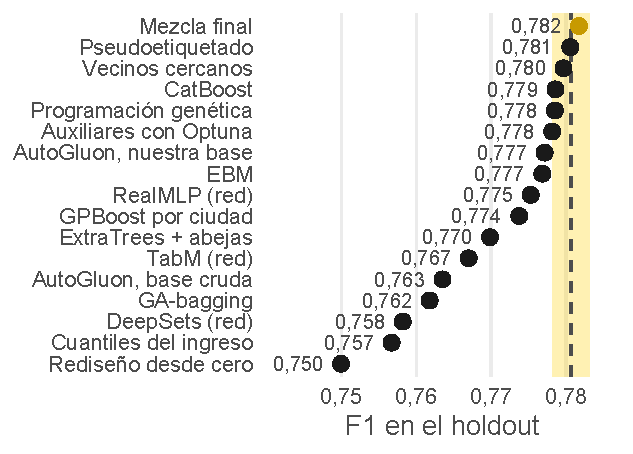
\includegraphics[height=5.3cm]{busqueda_techo}
    \column{0.34\textwidth}
      \footnotesize
      \textbf{Efecto mínimo detectable:} la mejora más pequeña que el holdout distingue del
      ruido es $\pm 0{,}0025$ (banda amarilla alrededor de LightGBM base, línea punteada).
      \begin{itemize}
        \item Ningún algoritmo nuevo supera a LightGBM.
        \item La mezcla final gana $+0{,}0007$ en CV repetida, IC 95\,\%
          [$+0{,}0002$; $+0{,}0012$]. Corrigiendo por la dependencia entre folds, el IC
          incluye cero.
      \end{itemize}
  \end{columns}
  \takeaway{Las mejoras posibles están por debajo de lo que los datos permiten detectar.}
  \fuente{F1 en holdout. Fuente: views/tablas/nivel7/ (etapa7\_b, etapa8 a etapa18); efecto mínimo de etapa16\_fase1\_resumen.csv.}
  \note{
    \textbf{Qué decir.} Probamos redes tabulares, AutoML, CatBoost, efectos aleatorios por
    ciudad, vecinos cercanos, programación genética de variables, pseudoetiquetado y un
    rediseño desde cero. Todos caen dentro o por debajo de la banda de ruido.\\[3pt]
    \textbf{Pregunta difícil: ¿por qué no quedarse con LightGBM solo?} Es nuestra
    recomendación práctica. La mezcla es la única que cumplió la regla fijada antes de la
    corrida (IC pareado sin cero en CV repetida y holdout no peor), pero gana milésimas y
    no sobrevive a la corrección por dependencia.
  }
\end{frame}

\begin{frame}{El techo está en los datos: sin el ingreso, un tercio de los pobres es indistinguible}
  \centering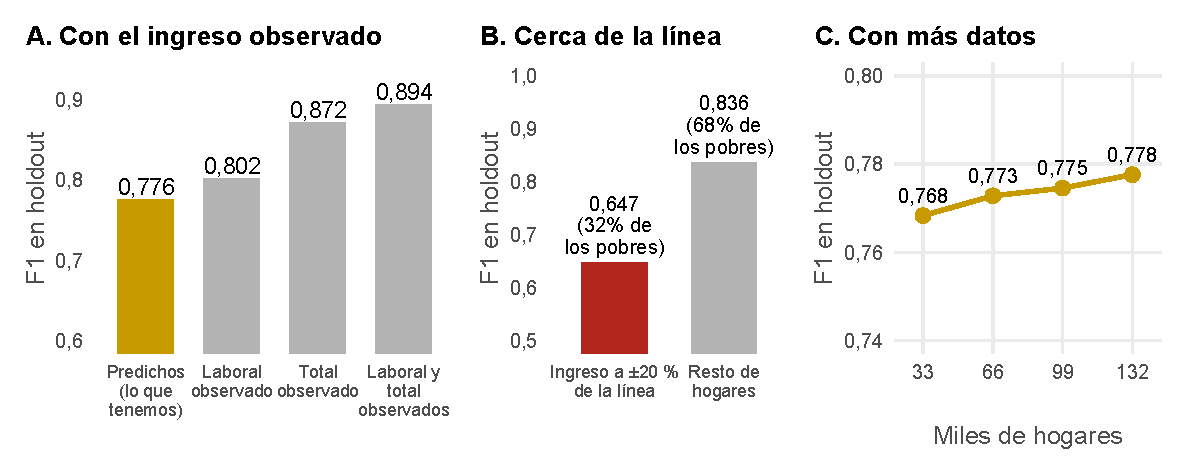
\includegraphics[height=3.85cm]{techo_tres_paneles}\par
  \raggedright\footnotesize
  \begin{columns}[T]
    \column{0.38\textwidth} \textbf{A.} Con el ingreso observado, el mismo modelo llegaría a 0,87--0,89.
    \column{0.30\textwidth} \textbf{B.} El 32\,\% de los pobres está a $\pm$\,20\,\% de la línea; ahí el F1 es 0,647.
    \column{0.28\textwidth} \textbf{C.} Cuadruplicar los datos sube el F1 solo 0,009.
  \end{columns}
  \takeaway{El límite viene sobre todo de la información que falta: el ingreso.}
  \fuente{Versión previa del modelo (LightGBM con auxiliares laboral y total), holdout. Fuente: views/tablas/nivel7/techo\_oraculo.csv, techo\_bandas.csv, techo\_curva\_aprendizaje.csv.}
  \note{
    \textbf{Qué decir.} Tres pruebas de que el techo es de información. Con el ingreso
    real, el F1 subiría a casi 0,9: el error que queda es el de predecir el ingreso. Ese
    error pesa cerca de la línea, donde está un tercio de los pobres y el F1 cae a 0,65. Y
    más datos casi no ayudan: la curva de aprendizaje es plana.\\[3pt]
    \textbf{Pregunta difícil: ¿por qué el oráculo no da F1 = 1?} Porque el ingreso de las
    personas no incluye el arriendo imputado a propietarios, que sí entra en el ingreso
    del hogar que define la pobreza.
  }
\end{frame}

%% ============================================================
\section{Implicaciones de política}
%% ============================================================
\begin{frame}{Excluimos al 18\,\% de los pobres, sobre todo a los más cercanos a la línea}
  \begin{columns}[c]
    \column{0.58\textwidth}
      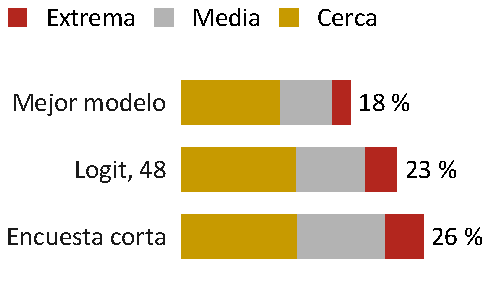
\includegraphics[width=\linewidth]{excluidos_por_modelo}
    \column{0.40\textwidth}
      \footnotesize
      \begin{itemize}
        \item \textbf{Subcobertura} 18,2\,\% (1.201 de 6.605 pobres). Brecha media de los
          excluidos: 0,22, frente a 0,37 del pobre promedio.
        \item \textbf{Filtración} 25,1\,\%, pero los no pobres incluidos están cerca: distancia
          media a la línea 0,51 (el no pobre promedio: 2,83).
        \item Más subcobertura en hogares de 1 y 2 personas (34\,\% y 28\,\%), Manizales
          (36\,\%) y Pereira (29\,\%).
      \end{itemize}
  \end{columns}
  \takeaway{Ponderando cada error por su distancia a la línea, la subcobertura baja a 11,2\,\% y la filtración a 1,2\,\%.}
  \fuente{Holdout, umbral 0,36; brecha $=1-$ingreso/línea. Mezcla sin el modelo limpio (95\,\% del peso del final). Fuente: views/tablas/nivel7/etapa15\_pesos\_bienestar.csv, etapa15\_errores\_subgrupo.csv.}
  \note{
    \textbf{Qué decir.} El F1 trata igual todos los errores, pero no cuestan lo mismo. El
    59\,\% de los pobres que dejamos fuera tiene ingreso de al menos 0,8 veces la línea, y
    los no pobres incluidos también están cerca. Ponderando cada error por su distancia a
    la línea, la subcobertura baja de 18 a 11\,\%.\\[3pt]
    \textbf{Pregunta difícil: ¿hay sesgo contra hogares pequeños?} Sí hay más
    subcobertura en hogares de 1 y 2 personas: su ingreso depende de una sola persona y es
    más difícil de predecir. Una agencia podría fijar un umbral más bajo para ese grupo.
  }
\end{frame}

\begin{frame}{Una encuesta corta excluye a más pobres, y a más pobres extremos}
  \begin{columns}[c]
    \column{0.52\textwidth}
      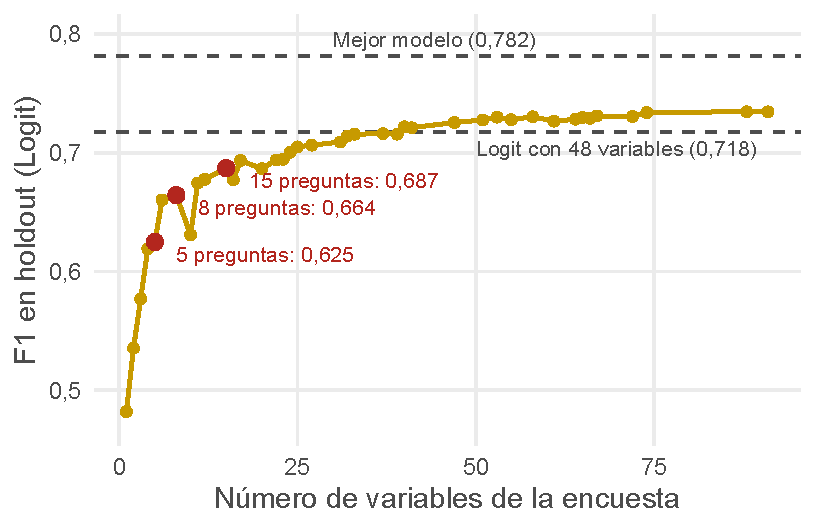
\includegraphics[width=\linewidth]{frontera_encuesta}
    \column{0.46\textwidth}
      \footnotesize
      \textbf{Intuición.} El mejor modelo necesita el módulo laboral de cada persona: es
      largo y autorreportado.
      \begin{itemize}
        \item Logit con las 8 mejores preguntas (ocupados, horas, cotizantes, quién quiere
          más horas, arriendo pagado y recibido, dormitorios): F1 0,664 frente a 0,782.
        \item Subcobertura 26,0\,\% y filtración 39,8\,\%.
        \item El 16\,\% de sus excluidos está en pobreza extrema (11\,\% con el mejor modelo).
      \end{itemize}
  \end{columns}
  \takeaway{Acortar la encuesta ahorra costo, pero corre la exclusión hacia los más pobres.}
  \fuente{Preguntas elegidas con NSGA-II (algoritmo genético con dos objetivos: F1 y número de preguntas). Fuente: views/tablas/nivel7/frontera\_encuesta\_corta.csv, etapa15\_pesos\_bienestar.csv.}
  \note{
    \textbf{Qué decir.} Buscamos el mejor conjunto de preguntas para cada tamaño de
    encuesta. Con 8 preguntas el F1 baja de 0,78 a 0,66, y lo más grave es a quiénes
    excluye: la exclusión se corre hacia la pobreza extrema.\\[3pt]
    \textbf{Pregunta difícil: ¿no pueden usar el modelo de ingreso en la encuesta corta?}
    No sin el módulo laboral: el auxiliar se alimenta de la ocupación, horas y cotización
    de cada persona. Por eso la frontera se construyó sin auxiliares.
  }
\end{frame}

\begin{frame}{El umbral es una decisión de política: la agencia puede comprar cobertura}
  \begin{columns}[c]
    \column{0.50\textwidth}
      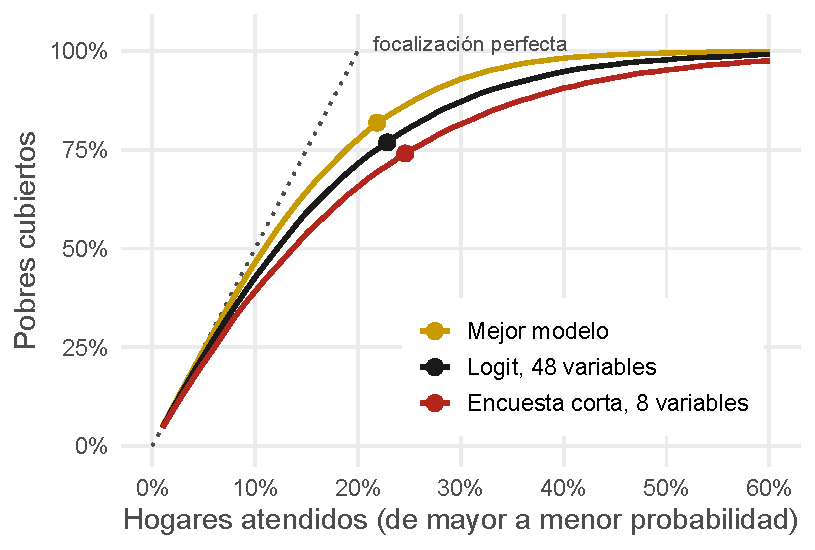
\includegraphics[width=\linewidth]{curva_cobertura_slides}
    \column{0.48\textwidth}
      \footnotesize
      \textbf{El umbral que maximiza F1 supone que ambos errores cuestan igual.}
      \begin{itemize}
        \item Atendiendo al 25\,\% de los hogares se cubre al 86,8\,\% de los pobres; al
          30\,\%, al 92,9\,\%.
        \item Bajar el umbral de 0,38 a 0,21 reduce la subcobertura de 19,3\,\% a 9,7\,\%;
          la filtración sube de 26,5\,\% a 36,2\,\% y el F1 apenas cae (0,769 a 0,747).
        \item La encuesta corta necesita atender al 40\,\% para cubrir al 90,6\,\%.
      \end{itemize}
  \end{columns}
  \takeaway{Si excluir a un pobre cuesta más que incluir a un no pobre, conviene bajar el umbral.}
  \fuente{Puntos: umbral elegido con OOF. Fuente: views/tablas/nivel7/etapa15\_curva\_cobertura.csv (holdout); views/tablas/escenarios\_politica\_n7.csv (OOF de la versión previa con auxiliares laboral y total).}
  \note{
    \textbf{Qué decir.} El F1 pondera igual los dos errores. Una agencia que valora más no
    dejar pobres por fuera puede bajar el umbral: la subcobertura se reduce a la mitad
    con 10 puntos más de filtración. Como los filtrados están cerca de la línea, ese costo
    es bajo en bienestar.\\[3pt]
    \textbf{Pregunta difícil: ¿qué umbral recomiendan?} Depende del costo relativo que
    fije la política. Con costos iguales, el del F1; si excluir cuesta el doble, uno más
    bajo. Es una decisión normativa, no estadística.
  }
\end{frame}

\begin{frame}{Recomendación a la agencia: medir bien el trabajo de cada persona}
  \small
  \begin{enumerate}
    \item \textbf{Con módulo laboral por persona:} modelo de ingreso por persona +
      LightGBM. Un LightGBM solo rinde igual que la mezcla y es más fácil de mantener.
    \item \textbf{Umbral según el costo de excluir, no según F1:} con un umbral menor la
      subcobertura baja de 19\,\% a 10\,\%, a cambio de filtración cerca de la línea.
    \item \textbf{Con presupuesto solo para encuesta corta:} usarla como filtro amplio
      (atender al 40\,\% cubre al 91\,\% de los pobres) y verificar con la encuesta larga a
      quienes quedan cerca del umbral.
    \item \textbf{Vigilar los grupos con más subcobertura:} hogares de 1--2 personas,
      Manizales y Pereira.
    \item \textbf{No esperar más de más modelos:} el techo es de información.
  \end{enumerate}
  \takeaway{El valor está en medir el ingreso; el algoritmo es secundario.}
  \note{
    \textbf{Qué decir.} Cinco recomendaciones que se siguen de la evidencia: el modelo
    sirve si se puede preguntar por el trabajo de cada persona; el umbral es una decisión
    de política; una encuesta corta funciona como primer filtro si se acepta más
    filtración; hay grupos que vigilar; y el límite es de información.\\[3pt]
    \textbf{Pregunta difícil: ¿son verificables las variables clave?} En parte. Tenencia
    y arriendo se pueden observar en una visita; horas e ingresos son autorreportados.
    Por eso recomendamos verificar en campo a los hogares cercanos al umbral, donde el
    modelo es menos confiable.
  }
\end{frame}

%% ============================================================
%% Apéndice
%% ============================================================
\appendix
\diapositivaglosario

\begin{frame}{Apéndice: auditoría de los datos, sin fuga ni errores de construcción}
  \small
  \begin{columns}[T]
    \column{0.48\textwidth}
      \textbf{Construcción}
      \begin{itemize}
        \item 0 personas sin hogar; 0 hogares sin jefe o con varios jefes.
        \item Pobre $=$ (ingreso per cápita $<$ línea) en los 164.960 hogares.
        \item Ids de train y test sin intersección.
      \end{itemize}
    \column{0.48\textwidth}
      \textbf{Fuga y cambio de distribución}
      \begin{itemize}
        \item Validación adversarial (¿se distingue train de test?): AUC 0,501 con las
          variables observadas; 0,713 con los auxiliares, por su ajuste completo en test.
        \item Reponderar por esa diferencia no cambia el F1 (IC con cero).
      \end{itemize}
  \end{columns}
  \fuente{Fuente: views/tablas/nivel7/forense\_resumen.csv, forense\_adversarial.csv, forense\_experimentos.csv.}
  \note{Respaldo para preguntas sobre fuga o cambio de distribución.}
\end{frame}

\begin{frame}{Apéndice: en CV repetida ninguna alternativa mejora de forma detectable}
  \centering\scriptsize
  \begin{tabular}{@{}lccc@{}}
    \toprule
    Candidato & F1 CV repetida (EE) & $\Delta$ vs.\ LightGBM [IC 95\,\%] & F1 holdout [IC 95\,\%] \\
    \midrule
    LightGBM base & 0,7752 (0,0008) & & 0,7806 [0,7731; 0,7885] \\
    + redes (mezcla sin limpio) & 0,7758 (0,0008) & $+0{,}0006$ [$-0{,}0001$; $+0{,}0013$] & 0,7820 [0,7743; 0,7897] \\
    \textbf{+ redes + limpio (final)} & \textbf{0,7759 (0,0008)} & $+0{,}0007$ [$+0{,}0002$; $+0{,}0012$] & 0,7817 [0,7742; 0,7894] \\
    CatBoost & 0,7722 (0,0007) & $-0{,}0030$ [$-0{,}0042$; $-0{,}0018$] & 0,7786 [0,7707; 0,7864] \\
    Base con códigos corregidos & 0,7754 (0,0008) & $+0{,}0002$ [$-0{,}0002$; $+0{,}0005$] & 0,7797 [0,7720; 0,7875] \\
    Rediseño desde cero & 0,7478 (0,0008) & $-0{,}0274$ [$-0{,}0289$; $-0{,}0260$] & 0,7499 [0,7420; 0,7581] \\
    \bottomrule
  \end{tabular}
  \fuente{IC pareados ingenuos (15 pares). Con la corrección de Nadeau y Bengio el IC del modelo final es [$-0{,}0004$; $+0{,}0017$]. Fuente: views/tablas/nivel7/etapa16\_fase1\_resumen.csv, etapa18\_resumen.csv.}
  \note{Respaldo: la única diferencia cuyo IC ingenuo excluye cero es la del modelo final, y por milésimas.}
\end{frame}

\begin{frame}{Apéndice: un rediseño desde cero llega a 0,750; le falta el ingreso por persona}
  \small
  \begin{itemize}
    \item Rehicimos el pipeline sin mirar el trabajo previo: 74 variables de hogar a partir
      del diccionario del DANE, con los códigos de ``no sabe'' como faltantes.
    \item Una variante con el ingreso del hogar como objetivo auxiliar (anidado) no mejora.
    \item F1 en CV repetida 0,748 y holdout 0,750, frente a 0,775 y 0,781 de LightGBM base;
      correlación de sus predicciones con LightGBM: 0,94.
    \item Lo que separa a los dos pipelines es predecir el ingreso de cada persona, no el
      del hogar.
  \end{itemize}
  \fuente{Fuente: limpio/resultados/; views/tablas/nivel7/etapa18\_resumen.csv.}
  \note{Respaldo: el rediseño confirma que el auxiliar a nivel persona es la pieza clave.}
\end{frame}

\end{document}
"
%% ============================================================
\documentclass[aspectratio=169,11pt]{beamer}
%% Preamble: packages and theme. Keep design changes in beamerthemeUniandes.sty
\usepackage[utf8]{inputenc}
\usepackage[T1]{fontenc}
\usepackage[spanish,es-nodecimaldot,es-noshorthands]{babel}
\usepackage{amsmath,amssymb}
\usepackage{graphicx}
\usepackage{booktabs}
\usepackage[round]{natbib}
\usetheme{Uniandes}

%% ---- Agregados para el Problem Set 2 (no cambian el diseño) ----
% Algunas instalaciones de MiKTeX no registran el mapa de Source Sans; se carga aquí.
\pdfmapfile{+SourceSansThree.map}
\usepackage{array}
\usepackage{xspace}
\usetikzlibrary{positioning,arrows.meta,decorations.pathreplacing}
\graphicspath{{../figuras/}{../../../views/figuras/}{../../../views/figuras/nivel7/}}

% Notas del presentador: el PDF de entrega no las muestra; la versión *_notas
% se compila con \def\connotas{} antes del documento y las intercala.
\ifdefined\connotas
  \setbeameroption{show notes}
\else
  \setbeameroption{hide notes}
\fi
\setbeamerfont{note page}{size=\small}
\setbeamertemplate{note page}{%
  \vspace{0.3cm}\insertslideintonotes{0.25}\par\vspace{0.2cm}
  \begin{minipage}{0.95\textwidth}\insertnote\end{minipage}}

% F1 público de Kaggle del mejor modelo (n18), tal como lo muestra la Overview.
\def\kagglepublico{0,78}

% Tabla pequeña con letra reducida
\newcommand{\tablachica}{\footnotesize\renewcommand{\arraystretch}{1.12}}
% Fuente de una figura o tabla, al pie
\newcommand{\fuente}[1]{\par\vspace{2pt}{\tiny\color{andesgray}#1\par}}
% Títulos sin cortar palabras con guion: se hace dentro de la plantilla del título
% (beamerthemeUniandes.sty), porque el minipage del título reinicia la alineación.
% Cajas de los diagramas sin guiones
\tikzset{every node/.append style={execute at begin node={\hyphenpenalty=10000\exhyphenpenalty=10000}}}

%% ============================================================
%%  Piezas comunes a los dos decks: Best Model Overview y glosario
%% ============================================================

% ---- Best Model Overview (diapositiva obligatoria, primera de cada deck) ----
\newcommand{\diapositivaoverview}{%
\begin{frame}{Best Model Overview}
  {Ingreso predicho por persona + LightGBM \;|\; Equipo 06, MECA 4107}
  \vspace{-0.1cm}
  \begin{columns}[T]
    \column{0.37\textwidth}\centering \keyfig{\kagglepublico}{F1 público en Kaggle}
    \column{0.30\textwidth}\centering \keyfig{0,782}{F1 en holdout, IC 95\,\% [0,774; 0,789]}
    \column{0.30\textwidth}\centering \keyfig{0,776}{F1 en CV repetida (15 evaluaciones)}
  \end{columns}
  \vspace{0.15cm}
  \footnotesize
  \begin{columns}[T]
    \column{0.49\textwidth}
      \textbf{Especificación}
      \begin{itemize}
        \item \textbf{Variable clave:} el ingreso de cada persona, predicho con lo que el test
          sí trae y sumado al hogar (1.324 variables en total).
        \item \textbf{Algoritmo:} LightGBM (76\,\%) mezclado con dos redes (19\,\%) y un
          rediseño desde cero (5\,\%); pesos elegidos fuera de muestra.
        \item \textbf{Regla:} pobre si $P(\text{pobre}) \geq 0{,}36$.
      \end{itemize}
    \column{0.49\textwidth}
      \textbf{Mensajes}
      \begin{enumerate}
        \item Las variables aportaron \textbf{9 veces más} F1 que los algoritmos.
        \item El techo (${\approx}\,0{,}78$) viene sobre todo de la información que falta.
        \item Excluye al 18\,\% de los pobres, casi todos cerca de la línea.
      \end{enumerate}
  \end{columns}
  \fuente{F1: media armónica de precisión y recall de la clase pobre. Holdout: 20\,\% del train nunca usado para decidir. Fuente: views/tablas/nivel7/etapa18\_resumen.csv.}
  \note{
    \textbf{Qué decir (1 min).} Nuestro mejor modelo clasifica hogares pobres con F1 de
    0,782 en datos que nunca usamos para decidir. La pieza clave no es el algoritmo sino
    una variable: predecimos cuánto gana cada persona con lo que el test sí trae
    (ocupación, horas, cotización) y lo sumamos al hogar. Tres mensajes: las variables
    pesan 9 veces más que el algoritmo, hay un techo que viene de los datos y los errores
    se concentran cerca de la línea.\\[3pt]
    \textbf{Pregunta difícil: ¿por qué una mezcla y no un solo modelo?} La mezcla gana
    +0,0007 en CV repetida frente a LightGBM solo. El IC ingenuo [+0,0002; +0,0012] excluye
    cero; el corregido por dependencia entre folds no. Es una mejora marginal: en la
    práctica LightGBM solo rinde igual.
  }
\end{frame}}

% ---- Glosario (apéndice de ambos decks, dos diapositivas) ----
\newcommand{\filaglosario}[2]{\textbf{#1} & #2 \\}
\newcommand{\diapositivaglosario}{%
\begin{frame}{Glosario (1/2): métricas y errores}
  \footnotesize\renewcommand{\arraystretch}{1.25}
  \begin{tabular}{@{}p{0.2\textwidth}p{0.76\textwidth}@{}}
    \toprule
    \filaglosario{Precisión}{De los hogares que el programa atiende, qué parte es pobre. $1-$precisión $=$ \textbf{filtración}: no pobres que reciben el beneficio.}
    \filaglosario{Recall}{De los hogares pobres, qué parte atiende el programa. $1-$recall $=$ \textbf{subcobertura}: pobres excluidos.}
    \filaglosario{F1}{Media armónica de precisión y recall: solo es alta si ambas lo son. No premia a los no pobres bien clasificados.}
    \filaglosario{Umbral}{Probabilidad a partir de la cual un hogar se clasifica como pobre. Bajarlo cubre más pobres a cambio de más filtración.}
    \filaglosario{IC 95\,\%}{Rango de valores compatibles con los datos. Si el IC de una diferencia incluye cero, no podemos afirmar que haya mejora.}
    \filaglosario{Efecto mínimo detectable}{La mejora más pequeña que el diseño detectaría con probabilidad 0,8.}
    \bottomrule
  \end{tabular}
  \note{Glosario de apoyo; se muestra solo si lo preguntan.}
\end{frame}
\begin{frame}{Glosario (2/2): validación y variables}
  \footnotesize\renewcommand{\arraystretch}{1.25}
  \begin{tabular}{@{}p{0.2\textwidth}p{0.76\textwidth}@{}}
    \toprule
    \filaglosario{Holdout}{20\,\% del train (32.993 hogares) apartado al inicio; solo se usa para medir, nunca para decidir.}
    \filaglosario{Validación cruzada}{El 80\,\% restante se parte en 5 bloques (folds): se entrena con 4 y se evalúa en el quinto, rotando.}
    \filaglosario{Fuera de fold (OOF)}{La predicción de cada hogar hecha por un modelo que no lo vio. Con ella se eligen umbral, pesos e hiperparámetros.}
    \filaglosario{CV repetida}{La validación cruzada repetida con 3 particiones nuevas: 15 evaluaciones para medir la variabilidad.}
    \filaglosario{Auxiliar de ingreso}{Modelo que predice el ingreso de cada persona con variables que el test sí trae; sumado al hogar, entra como variable.}
    \filaglosario{OOF anidada}{El auxiliar que alimenta a un hogar no vio ese hogar ni su fold de validación: así no se filtra la respuesta.}
    \bottomrule
  \end{tabular}
  \note{Glosario de apoyo; se muestra solo si lo preguntan.}
\end{frame}}


\title[Predicting Poverty: Best Model Deep Dive]{Predicting Poverty: Best Model Deep Dive}
\author[Labastidas y Garcia | Equipo 06]{Esteban David Labastidas Martínez \and Neislen Stiven Garcia Silva}
\institute{Facultad de Economía\\ Universidad de los Andes}
\date[Oct 2026]{Bogotá, octubre de 2026}

\begin{document}
\andessectionslidesfalse

%% 1. Best Model Overview (obligatoria)
\diapositivaoverview

%% ============================================================
\section{Datos}
%% ============================================================
\begin{frame}{El test no trae ingresos: hay que inferir la pobreza sin ver su definición}
  \begin{columns}[T]
    \column{0.62\textwidth}
      \small
      \textbf{Intuición.} Un hogar es pobre si su ingreso per cápita está bajo la línea de
      pobreza de su ciudad y mes. El test no trae ningún ingreso.
      \begin{itemize}
        \item 79 variables solo existen en train, entre ellas todos los ingresos.
        \item Pobre $\Leftrightarrow$ ingreso per cápita $<$ línea, sin excepciones.
        \item Bogotá está en train pero no en test.
      \end{itemize}
      \textbf{Métrica.} ``Nadie es pobre'' acierta en el 80\,\% de los hogares, pero tiene
      F1 $=0$. El F1 combina \textbf{filtración} (no pobres atendidos) y
      \textbf{subcobertura} (pobres excluidos).
    \column{0.34\textwidth}
      \centering
      \keyfig{164.960}{hogares en train}\\[0.02cm]
      \keyfig{66.168}{hogares en test}\\[0.02cm]
      \keyfig{20,0\,\%}{hogares pobres}
  \end{columns}
  \takeaway{El problema es reconstruir el ingreso con lo que sí se observa.}
  \fuente{Fuente: views/tablas/nivel7/forense\_resumen.csv; views/tablas/desbalance\_clases.csv.}
  \note{
    \textbf{Qué decir.} La definición de pobreza es mecánica: ingreso per cápita contra la
    línea. El reto es que el test no trae ingresos, así que hay que inferirlos de lo
    observable. La clase pobre es una de cada cinco; por eso no usamos accuracy sino F1, que
    castiga tanto dejar pobres por fuera (subcobertura) como incluir no pobres
    (filtración).\\[3pt]
    \textbf{Pregunta difícil: ¿por qué no predecir el ingreso y aplicar la línea?} El
    enunciado pide clasificación. Usamos el ingreso solo como objetivo auxiliar por
    persona, nunca como predictor; el clasificador final predice la etiqueta.
  }
\end{frame}

\begin{frame}{La teoría acierta: trabajo, dependencia, educación y vivienda predicen la pobreza}
  \begin{columns}[c]
    \column{0.64\textwidth}
      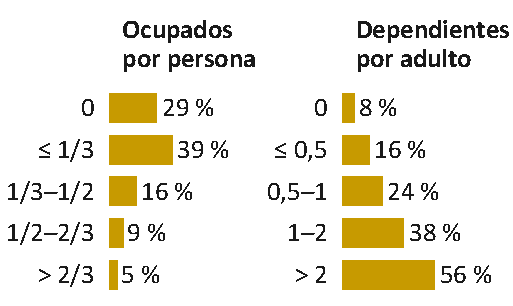
\includegraphics[width=\linewidth]{correlatos_pobreza}
    \column{0.34\textwidth}
      \footnotesize
      \textbf{Ingreso per cápita} $=$ cuántos trabajan $\times$ cuánto gana cada uno
      $\div$ cuántos comen.
      \begin{itemize}
        \item Más dependientes por adulto: pobreza de 8\,\% a 56\,\%.
        \item Jefe sin educación 40\,\%; con superior 8\,\%.
        \item Sin ocupados (29\,\%) es menos pobre que un tercio ocupado (39\,\%):
          pensiones y rentas.
      \end{itemize}
  \end{columns}
  \takeaway{Ninguna variable sola basta: la mejor regla de una variable da F1 de 0,473.}
  \fuente{Fuente: base de hogares de train (scripts/13\_figuras\_presentacion.R); views/tablas/leaderboard\_interno.csv.}
  \note{
    \textbf{Qué decir.} Partimos de la identidad del ingreso: cuántos trabajan, cuánto gana
    cada uno y entre cuántos se reparte. Los datos confirman cada pieza. Un patrón rompe el
    prior: los hogares sin ocupados no son los más pobres, porque muchos viven de pensiones
    o rentas. La relación no es lineal.\\[3pt]
    \textbf{Pregunta difícil: ¿basta con estas variables en un Logit?} No: un Logit con 5
    variables teóricas da F1 de 0,457, por debajo de la mejor regla de una variable
    (0,473). Con 48 variables construidas desde las personas sube a 0,718.
  }
\end{frame}

%% ============================================================
\section{Mejor modelo}
%% ============================================================
\begin{frame}{Confiamos en el holdout porque nunca se usó para decidir}
  \centering
  \begin{tikzpicture}[x=1cm,y=1cm,font=\scriptsize]
    \foreach \i in {0,...,4} {
      \fill[andeslight] (\i*1.9,0) rectangle ++(1.8,0.7);
      \pgfmathtruncatemacro{\k}{\i+1}
      \node at (\i*1.9+0.9,0.35) {fold \k};
    }
    \fill[andesaccent!35] (9.6,0) rectangle ++(2.6,0.7);
    \node at (10.9,0.35) {\textbf{holdout} 20\,\%};
    \draw[decorate,decoration={brace,amplitude=4pt}] (0,0.82) -- (9.4,0.82)
      node[midway,above=4pt] {80\,\% = 131.967 hogares: validación cruzada (CV) de 5 folds};
    \draw[decorate,decoration={brace,amplitude=4pt}] (9.6,0.82) -- (12.2,0.82)
      node[midway,above=4pt] {32.993 hogares};
    \node[draw=andesmid,rounded corners,fill=white,text width=6.2cm,align=left] (oof) at (4.7,-1.05)
      {Cada hogar recibe una predicción \textbf{fuera de fold (OOF)}, de un modelo que no lo
       vio. Con la OOF se eligen hiperparámetros, \textbf{umbral} y pesos de mezcla.};
    \node[draw=andesmid,rounded corners,fill=white,text width=3.2cm,align=left] (ho) at (10.9,-1.05)
      {Se mide una sola vez, con el umbral ya fijo.};
    \draw[-{Latex},andesgray] (4.7,-0.05) -- (oof.north);
    \draw[-{Latex},andesgray] (10.9,-0.05) -- (ho.north);
  \end{tikzpicture}
  \vspace{0.15cm}

  \raggedright\small
  \textbf{CV repetida:} al final repetimos la CV con 3 particiones nuevas (15 evaluaciones) y
  comparamos modelos con intervalos de confianza (IC: rango de valores compatibles con los datos) pareados por fold y por remuestra del holdout.
  \takeaway{La CV repetida reproduce la original casi al milésimo: 0,7752 frente a 0,7748.}
  \fuente{Fuente: views/tablas/resumen\_particion.csv; views/tablas/nivel7/etapa16\_fase1\_resumen.csv.}
  \note{
    \textbf{Qué decir.} Apartamos un 20\,\% al inicio y no lo tocamos. Todo lo que se
    elige (hiperparámetros, umbral, pesos) se elige con predicciones fuera de fold: cada
    hogar es predicho por un modelo que no lo vio. Al final repetimos la validación con
    tres particiones nuevas para medir cuánto ruido hay en una diferencia.\\[3pt]
    \textbf{Pregunta difícil: ¿no se sobreajustó el holdout tras muchas etapas?} Lo
    miramos muchas veces, aunque nunca para elegir parámetros. Por eso la comparación
    final usa la CV repetida en particiones nuevas, donde el orden de los candidatos se
    mantiene. Kaggle es la verificación externa.
  }
\end{frame}

\begin{frame}{Las variables aportaron 9 veces más F1 que el cambio de algoritmo}
  \begin{columns}[c]
    \column{0.66\textwidth}
      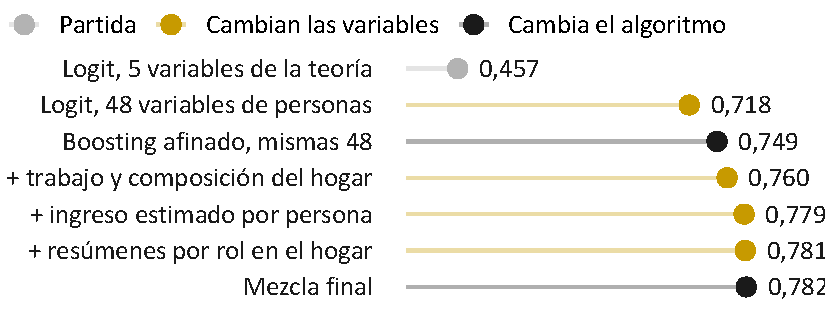
\includegraphics[width=\linewidth]{escalera_completa}
    \column{0.32\textwidth}
      \small
      \textbf{Suma de los saltos}
      \begin{itemize}
        \item \textcolor{andesaccent}{\textbf{Variables}}: $+0{,}292$.
        \item \textbf{Algoritmo}: $+0{,}032$.
      \end{itemize}
      El salto mayor (0,457 $\to$ 0,718) es el mismo Logit con variables construidas desde
      las personas.
  \end{columns}
  \takeaway{Rinde más entender el hogar que cambiar de algoritmo.}
  \fuente{F1 en holdout. Fuente: views/tablas/leaderboard\_interno.csv y nivel7/ (ablacion\_etapa1, resumen\_etapa2, etapa6\_ablacion, etapa7\_a, etapa18\_resumen).}
  \note{
    \textbf{Qué decir.} Cada punto es un paso de la escalera, medido en el mismo holdout.
    Los amarillos cambian las variables con el algoritmo fijo; los negros cambian el
    algoritmo con las variables fijas. Las variables suman 0,29 de F1; los algoritmos,
    0,03.\\[3pt]
    \textbf{Pregunta difícil: ¿la descomposición depende del orden?} Sí, es secuencial.
    Pero el contraste se sostiene en ambos sentidos: con 48 variables, pasar de Logit a
    XGBoost suma 0,029; con LightGBM fijo, pasar de 48 variables a la base final suma
    0,032; y otros algoritmos sobre la base final quedan entre 0,767 y 0,779.
  }
\end{frame}

\begin{frame}{El salto clave: predecir el ingreso de cada persona y sumarlo al hogar}
  \begin{columns}[c]
    \column{0.55\textwidth}
      \centering
      \begin{tikzpicture}[font=\scriptsize,
          caja/.style={draw=andesmid,rounded corners,fill=andeslight,text width=2.4cm,align=center,minimum height=0.8cm},
          clave/.style={caja,fill=andesyellow!45},
          flecha/.style={-{Latex},andesgray,thick}]
        \node[caja] (p) {Personas en train: ocupación, horas, cotización \textbf{+ su ingreso}};
        \node[clave,right=0.5cm of p] (m) {Modelo de ingreso por persona};
        \node[caja,below=0.45cm of m] (q) {Ingreso predicho de cada persona (también en test)};
        \node[caja,left=0.5cm of q] (h) {Suma del hogar $\div$ personas $\div$ línea};
        \node[clave,below=0.45cm of h] (c) {Clasificador del hogar};
        \draw[flecha] (p) -- (m);
        \draw[flecha] (m) -- (q);
        \draw[flecha] (q) -- (h);
        \draw[flecha] (h) -- (c);
      \end{tikzpicture}
    \column{0.43\textwidth}
      \tablachica
      \begin{tabular}{@{}lcc@{}}
        \toprule
        LightGBM con\ldots & F1 holdout & $\Delta$ \\
        \midrule
        sin auxiliares & 0,760 & \\
        + ingreso laboral & 0,771 & $+0{,}011$ \\
        + ingreso total & 0,776 & $+0{,}005$ \\
        + ingreso por fuente & 0,779 & $+0{,}003$ \\
        \bottomrule
      \end{tabular}
      \vspace{0.2cm}

      \footnotesize
      \textbf{OOF anidada:} el modelo de ingreso que alimenta a un hogar no vio ese hogar
      ni su fold de validación.
  \end{columns}
  \takeaway{El ingreso de train se usa como objetivo auxiliar, nunca como predictor.}
  \fuente{Fuente: views/tablas/nivel7/ablacion\_etapa1.csv, resumen\_etapa2.csv, etapa6\_ablacion.csv.}
  \note{
    \textbf{Qué decir.} En train sabemos cuánto gana cada persona. Entrenamos un modelo
    que predice ese ingreso con lo que el test sí trae. En test lo aplicamos, sumamos las
    predicciones del hogar y las dividimos por personas y por la línea. Solo el ingreso
    laboral predicho suma más de un punto de F1.\\[3pt]
    \textbf{Pregunta difícil: ¿no es fuga de información?} No, por construcción: cada
    hogar recibe la predicción de un modelo que no lo vio, y dentro de cada fold el
    auxiliar tampoco vio el fold de validación. Lo verifican tests automáticos. Con las
    1.306 variables observadas, un clasificador no distingue train de test (AUC 0,501);
    con los auxiliares sube a 0,713 porque en test se calculan con ajuste completo y en
    train fuera de fold.
  }
\end{frame}

\begin{frame}{El modelo decide con el ingreso predicho y con la vivienda}
  \begin{columns}[c]
    \column{0.60\textwidth}
      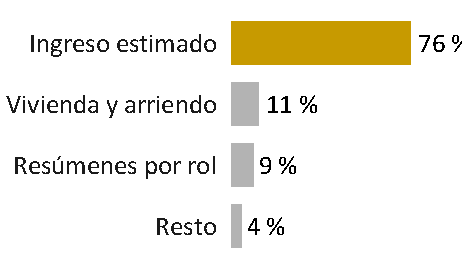
\includegraphics[width=\linewidth]{importancia_n7_a}
    \column{0.38\textwidth}
      \tablachica
      \begin{tabular}{@{}lrr@{}}
        \toprule
        Familia & Vars. & Ganancia \\
        \midrule
        Ingreso predicho & 17 & 75,6\,\% \\
        Vivienda y arriendo & 15 & 11,2\,\% \\
        Agregados por rol & 1.026 & 9,1\,\% \\
        Resto & 266 & 4,0\,\% \\
        \bottomrule
      \end{tabular}
      \vspace{0.15cm}

      \footnotesize
      En un boosting interpretable (EBM), la interacción más fuerte es arriendo por
      persona $\times$ vivienda propia pagada.
  \end{columns}
  \takeaway{El modelo reconstruye el ingreso y lo ajusta por el costo de la vivienda.}
  \fuente{Ganancia: reducción de la pérdida atribuida a cada variable en LightGBM (76\,\% de la mezcla). Fuente: views/tablas/nivel7/etapa7\_a\_importancia.csv, etapa15\_ebm\_importancia.csv.}
  \note{
    \textbf{Qué decir.} Tres cuartas partes de lo que aprende el modelo vienen de 17
    variables de ingreso predicho. Le sigue la vivienda: arriendo frente a la línea y
    tenencia. El arriendo revela capacidad de pago, y vivir en casa propia pagada es un
    ingreso implícito.\\[3pt]
    \textbf{Pregunta difícil: la ganancia favorece variables continuas.} Sí puede sesgar.
    Por eso lo contrastamos con un EBM, que mide el aporte medio al log-odds: también
    mandan el ingreso total predicho (0,57) y el arriendo por persona (0,50).
  }
\end{frame}

\begin{frame}{Los hiperparámetros importaron poco; el desbalance, nada}
  \begin{columns}[T]
    \column{0.52\textwidth}
      \tablachica
      \textbf{LightGBM}: 50 configuraciones (hipercubo latino), CV de 5 folds\\[3pt]
      \scriptsize
      \begin{tabular}{@{}lll@{}}
        \toprule
        Hiperparámetro & Valor & Lectura \\
        \midrule
        Rondas $\times$ tasa & 1.852 $\times$ 0,011 & aprende despacio \\
        Hojas por árbol & 31 & árboles pequeños \\
        Mínimo por hoja & 171 hogares & no memoriza \\
        Variables por corte & 82\,\% & algo de azar \\
        Hogares por árbol & 70\,\% & algo de azar \\
        \bottomrule
      \end{tabular}
    \column{0.44\textwidth}
      \footnotesize
      \begin{itemize}
        \item Reafinar con 75 intentos (Optuna) sobre las variables nuevas da el mismo F1:
          0,7759 frente a 0,7760.
        \item Promediar 5 semillas cambia el F1 en menos de 0,002.
        \item \textbf{Desbalance:} SMOTE, submuestreo y pesos de clase dan 0,745, 0,747 y
          0,744, frente a 0,746 sin balancear. Solo mueven el umbral óptimo (0,36 $\to$
          0,66 con pesos).
      \end{itemize}
  \end{columns}
  \takeaway{Elegir el umbral con OOF ya corrige el desbalance; rebalancear no agrega información.}
  \fuente{F1 en holdout. Fuente: views/tablas/leaderboard\_interno.csv; views/tablas/nivel7/resumen\_etapa2.csv.}
  \note{
    \textbf{Qué decir.} La configuración ganadora es conservadora: muchos árboles
    pequeños, aprendizaje lento y hojas de al menos 171 hogares. Buscar de nuevo con 75
    intentos no mejora. Rebalancear cambia la escala de las probabilidades, pero como el
    umbral se elige maximizando F1, el resultado es el mismo.\\[3pt]
    \textbf{Pregunta difícil: ¿por qué no tunear con el holdout?} Porque dejaría de ser
    una medida limpia. Todo el tuning usa F1 fuera de fold sobre el 80\,\%.
  }
\end{frame}

\begin{frame}{Dieciséis alternativas chocan con el mismo techo}
  \begin{columns}[c]
    \column{0.64\textwidth}
      \centering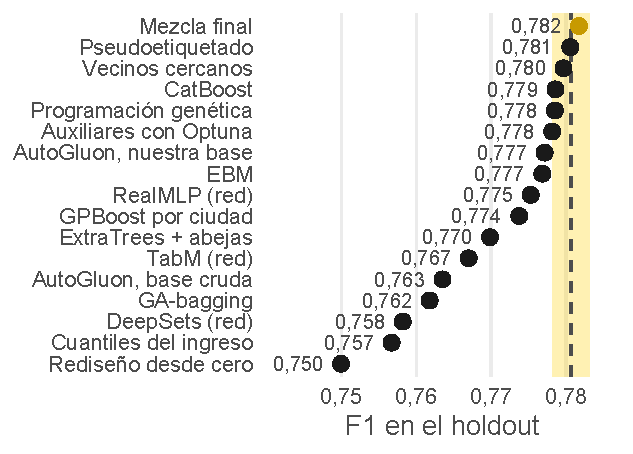
\includegraphics[height=5.3cm]{busqueda_techo}
    \column{0.34\textwidth}
      \footnotesize
      \textbf{Efecto mínimo detectable:} la mejora más pequeña que el holdout distingue del
      ruido es $\pm 0{,}0025$ (banda amarilla alrededor de LightGBM base, línea punteada).
      \begin{itemize}
        \item Ningún algoritmo nuevo supera a LightGBM.
        \item La mezcla final gana $+0{,}0007$ en CV repetida, IC 95\,\%
          [$+0{,}0002$; $+0{,}0012$]. Corrigiendo por la dependencia entre folds, el IC
          incluye cero.
      \end{itemize}
  \end{columns}
  \takeaway{Las mejoras posibles están por debajo de lo que los datos permiten detectar.}
  \fuente{F1 en holdout. Fuente: views/tablas/nivel7/ (etapa7\_b, etapa8 a etapa18); efecto mínimo de etapa16\_fase1\_resumen.csv.}
  \note{
    \textbf{Qué decir.} Probamos redes tabulares, AutoML, CatBoost, efectos aleatorios por
    ciudad, vecinos cercanos, programación genética de variables, pseudoetiquetado y un
    rediseño desde cero. Todos caen dentro o por debajo de la banda de ruido.\\[3pt]
    \textbf{Pregunta difícil: ¿por qué no quedarse con LightGBM solo?} Es nuestra
    recomendación práctica. La mezcla es la única que cumplió la regla fijada antes de la
    corrida (IC pareado sin cero en CV repetida y holdout no peor), pero gana milésimas y
    no sobrevive a la corrección por dependencia.
  }
\end{frame}

\begin{frame}{El techo está en los datos: sin el ingreso, un tercio de los pobres es indistinguible}
  \centering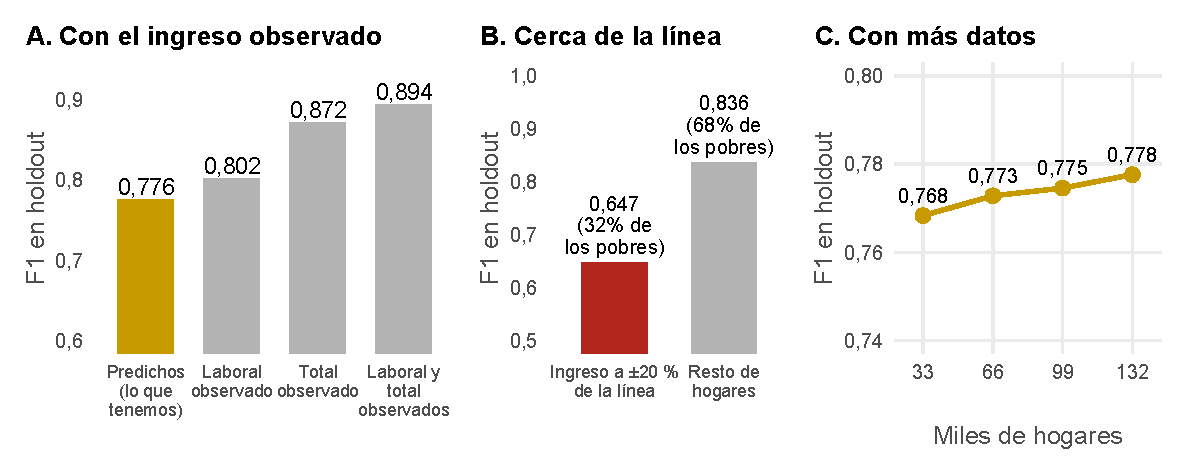
\includegraphics[height=3.85cm]{techo_tres_paneles}\par
  \raggedright\footnotesize
  \begin{columns}[T]
    \column{0.38\textwidth} \textbf{A.} Con el ingreso observado, el mismo modelo llegaría a 0,87--0,89.
    \column{0.30\textwidth} \textbf{B.} El 32\,\% de los pobres está a $\pm$\,20\,\% de la línea; ahí el F1 es 0,647.
    \column{0.28\textwidth} \textbf{C.} Cuadruplicar los datos sube el F1 solo 0,009.
  \end{columns}
  \takeaway{El límite viene sobre todo de la información que falta: el ingreso.}
  \fuente{Versión previa del modelo (LightGBM con auxiliares laboral y total), holdout. Fuente: views/tablas/nivel7/techo\_oraculo.csv, techo\_bandas.csv, techo\_curva\_aprendizaje.csv.}
  \note{
    \textbf{Qué decir.} Tres pruebas de que el techo es de información. Con el ingreso
    real, el F1 subiría a casi 0,9: el error que queda es el de predecir el ingreso. Ese
    error pesa cerca de la línea, donde está un tercio de los pobres y el F1 cae a 0,65. Y
    más datos casi no ayudan: la curva de aprendizaje es plana.\\[3pt]
    \textbf{Pregunta difícil: ¿por qué el oráculo no da F1 = 1?} Porque el ingreso de las
    personas no incluye el arriendo imputado a propietarios, que sí entra en el ingreso
    del hogar que define la pobreza.
  }
\end{frame}

%% ============================================================
\section{Implicaciones de política}
%% ============================================================
\begin{frame}{Excluimos al 18\,\% de los pobres, sobre todo a los más cercanos a la línea}
  \begin{columns}[c]
    \column{0.58\textwidth}
      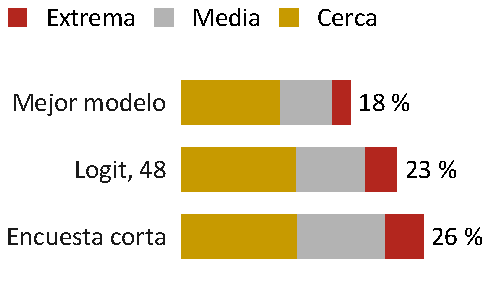
\includegraphics[width=\linewidth]{excluidos_por_modelo}
    \column{0.40\textwidth}
      \footnotesize
      \begin{itemize}
        \item \textbf{Subcobertura} 18,2\,\% (1.201 de 6.605 pobres). Brecha media de los
          excluidos: 0,22, frente a 0,37 del pobre promedio.
        \item \textbf{Filtración} 25,1\,\%, pero los no pobres incluidos están cerca: distancia
          media a la línea 0,51 (el no pobre promedio: 2,83).
        \item Más subcobertura en hogares de 1 y 2 personas (34\,\% y 28\,\%), Manizales
          (36\,\%) y Pereira (29\,\%).
      \end{itemize}
  \end{columns}
  \takeaway{Ponderando cada error por su distancia a la línea, la subcobertura baja a 11,2\,\% y la filtración a 1,2\,\%.}
  \fuente{Holdout, umbral 0,36; brecha $=1-$ingreso/línea. Mezcla sin el modelo limpio (95\,\% del peso del final). Fuente: views/tablas/nivel7/etapa15\_pesos\_bienestar.csv, etapa15\_errores\_subgrupo.csv.}
  \note{
    \textbf{Qué decir.} El F1 trata igual todos los errores, pero no cuestan lo mismo. El
    59\,\% de los pobres que dejamos fuera tiene ingreso de al menos 0,8 veces la línea, y
    los no pobres incluidos también están cerca. Ponderando cada error por su distancia a
    la línea, la subcobertura baja de 18 a 11\,\%.\\[3pt]
    \textbf{Pregunta difícil: ¿hay sesgo contra hogares pequeños?} Sí hay más
    subcobertura en hogares de 1 y 2 personas: su ingreso depende de una sola persona y es
    más difícil de predecir. Una agencia podría fijar un umbral más bajo para ese grupo.
  }
\end{frame}

\begin{frame}{Una encuesta corta excluye a más pobres, y a más pobres extremos}
  \begin{columns}[c]
    \column{0.52\textwidth}
      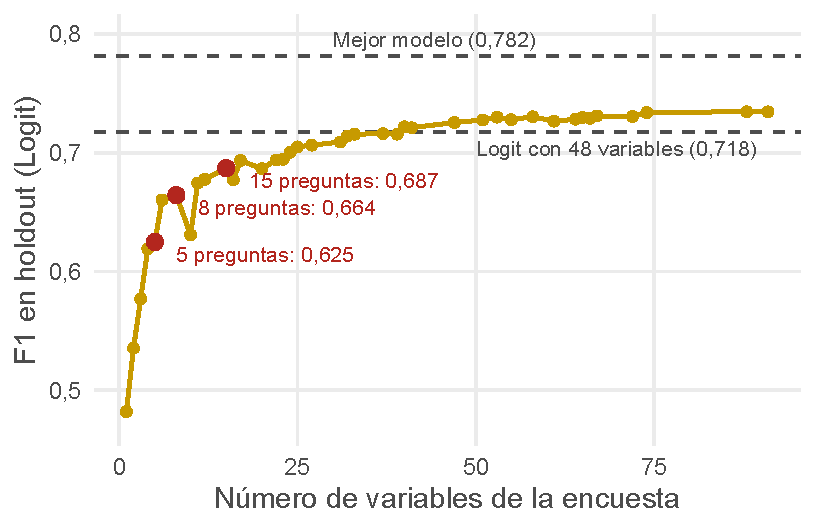
\includegraphics[width=\linewidth]{frontera_encuesta}
    \column{0.46\textwidth}
      \footnotesize
      \textbf{Intuición.} El mejor modelo necesita el módulo laboral de cada persona: es
      largo y autorreportado.
      \begin{itemize}
        \item Logit con las 8 mejores preguntas (ocupados, horas, cotizantes, quién quiere
          más horas, arriendo pagado y recibido, dormitorios): F1 0,664 frente a 0,782.
        \item Subcobertura 26,0\,\% y filtración 39,8\,\%.
        \item El 16\,\% de sus excluidos está en pobreza extrema (11\,\% con el mejor modelo).
      \end{itemize}
  \end{columns}
  \takeaway{Acortar la encuesta ahorra costo, pero corre la exclusión hacia los más pobres.}
  \fuente{Preguntas elegidas con NSGA-II (algoritmo genético con dos objetivos: F1 y número de preguntas). Fuente: views/tablas/nivel7/frontera\_encuesta\_corta.csv, etapa15\_pesos\_bienestar.csv.}
  \note{
    \textbf{Qué decir.} Buscamos el mejor conjunto de preguntas para cada tamaño de
    encuesta. Con 8 preguntas el F1 baja de 0,78 a 0,66, y lo más grave es a quiénes
    excluye: la exclusión se corre hacia la pobreza extrema.\\[3pt]
    \textbf{Pregunta difícil: ¿no pueden usar el modelo de ingreso en la encuesta corta?}
    No sin el módulo laboral: el auxiliar se alimenta de la ocupación, horas y cotización
    de cada persona. Por eso la frontera se construyó sin auxiliares.
  }
\end{frame}

\begin{frame}{El umbral es una decisión de política: la agencia puede comprar cobertura}
  \begin{columns}[c]
    \column{0.50\textwidth}
      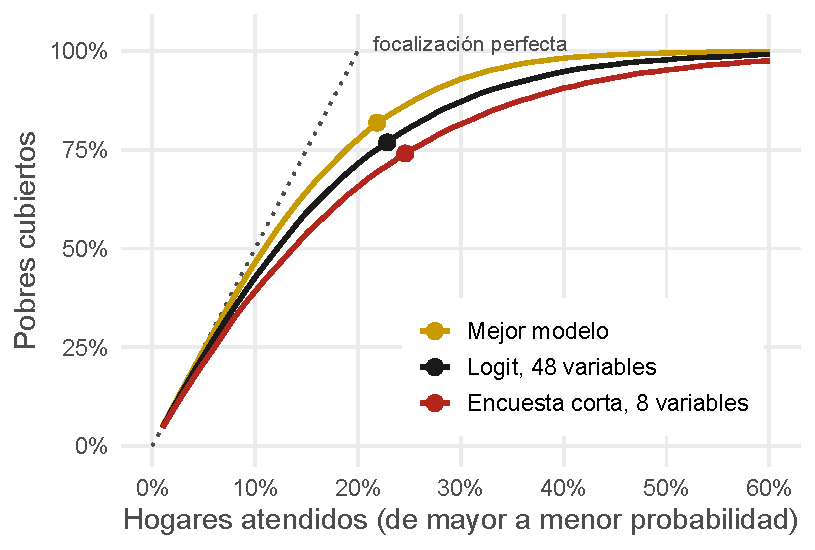
\includegraphics[width=\linewidth]{curva_cobertura_slides}
    \column{0.48\textwidth}
      \footnotesize
      \textbf{El umbral que maximiza F1 supone que ambos errores cuestan igual.}
      \begin{itemize}
        \item Atendiendo al 25\,\% de los hogares se cubre al 86,8\,\% de los pobres; al
          30\,\%, al 92,9\,\%.
        \item Bajar el umbral de 0,38 a 0,21 reduce la subcobertura de 19,3\,\% a 9,7\,\%;
          la filtración sube de 26,5\,\% a 36,2\,\% y el F1 apenas cae (0,769 a 0,747).
        \item La encuesta corta necesita atender al 40\,\% para cubrir al 90,6\,\%.
      \end{itemize}
  \end{columns}
  \takeaway{Si excluir a un pobre cuesta más que incluir a un no pobre, conviene bajar el umbral.}
  \fuente{Puntos: umbral elegido con OOF. Fuente: views/tablas/nivel7/etapa15\_curva\_cobertura.csv (holdout); views/tablas/escenarios\_politica\_n7.csv (OOF de la versión previa con auxiliares laboral y total).}
  \note{
    \textbf{Qué decir.} El F1 pondera igual los dos errores. Una agencia que valora más no
    dejar pobres por fuera puede bajar el umbral: la subcobertura se reduce a la mitad
    con 10 puntos más de filtración. Como los filtrados están cerca de la línea, ese costo
    es bajo en bienestar.\\[3pt]
    \textbf{Pregunta difícil: ¿qué umbral recomiendan?} Depende del costo relativo que
    fije la política. Con costos iguales, el del F1; si excluir cuesta el doble, uno más
    bajo. Es una decisión normativa, no estadística.
  }
\end{frame}

\begin{frame}{Recomendación a la agencia: medir bien el trabajo de cada persona}
  \small
  \begin{enumerate}
    \item \textbf{Con módulo laboral por persona:} modelo de ingreso por persona +
      LightGBM. Un LightGBM solo rinde igual que la mezcla y es más fácil de mantener.
    \item \textbf{Umbral según el costo de excluir, no según F1:} con un umbral menor la
      subcobertura baja de 19\,\% a 10\,\%, a cambio de filtración cerca de la línea.
    \item \textbf{Con presupuesto solo para encuesta corta:} usarla como filtro amplio
      (atender al 40\,\% cubre al 91\,\% de los pobres) y verificar con la encuesta larga a
      quienes quedan cerca del umbral.
    \item \textbf{Vigilar los grupos con más subcobertura:} hogares de 1--2 personas,
      Manizales y Pereira.
    \item \textbf{No esperar más de más modelos:} el techo es de información.
  \end{enumerate}
  \takeaway{El valor está en medir el ingreso; el algoritmo es secundario.}
  \note{
    \textbf{Qué decir.} Cinco recomendaciones que se siguen de la evidencia: el modelo
    sirve si se puede preguntar por el trabajo de cada persona; el umbral es una decisión
    de política; una encuesta corta funciona como primer filtro si se acepta más
    filtración; hay grupos que vigilar; y el límite es de información.\\[3pt]
    \textbf{Pregunta difícil: ¿son verificables las variables clave?} En parte. Tenencia
    y arriendo se pueden observar en una visita; horas e ingresos son autorreportados.
    Por eso recomendamos verificar en campo a los hogares cercanos al umbral, donde el
    modelo es menos confiable.
  }
\end{frame}

%% ============================================================
%% Apéndice
%% ============================================================
\appendix
\diapositivaglosario

\begin{frame}{Apéndice: auditoría de los datos, sin fuga ni errores de construcción}
  \small
  \begin{columns}[T]
    \column{0.48\textwidth}
      \textbf{Construcción}
      \begin{itemize}
        \item 0 personas sin hogar; 0 hogares sin jefe o con varios jefes.
        \item Pobre $=$ (ingreso per cápita $<$ línea) en los 164.960 hogares.
        \item Ids de train y test sin intersección.
      \end{itemize}
    \column{0.48\textwidth}
      \textbf{Fuga y cambio de distribución}
      \begin{itemize}
        \item Validación adversarial (¿se distingue train de test?): AUC 0,501 con las
          variables observadas; 0,713 con los auxiliares, por su ajuste completo en test.
        \item Reponderar por esa diferencia no cambia el F1 (IC con cero).
      \end{itemize}
  \end{columns}
  \fuente{Fuente: views/tablas/nivel7/forense\_resumen.csv, forense\_adversarial.csv, forense\_experimentos.csv.}
  \note{Respaldo para preguntas sobre fuga o cambio de distribución.}
\end{frame}

\begin{frame}{Apéndice: en CV repetida ninguna alternativa mejora de forma detectable}
  \centering\scriptsize
  \begin{tabular}{@{}lccc@{}}
    \toprule
    Candidato & F1 CV repetida (EE) & $\Delta$ vs.\ LightGBM [IC 95\,\%] & F1 holdout [IC 95\,\%] \\
    \midrule
    LightGBM base & 0,7752 (0,0008) & & 0,7806 [0,7731; 0,7885] \\
    + redes (mezcla sin limpio) & 0,7758 (0,0008) & $+0{,}0006$ [$-0{,}0001$; $+0{,}0013$] & 0,7820 [0,7743; 0,7897] \\
    \textbf{+ redes + limpio (final)} & \textbf{0,7759 (0,0008)} & $+0{,}0007$ [$+0{,}0002$; $+0{,}0012$] & 0,7817 [0,7742; 0,7894] \\
    CatBoost & 0,7722 (0,0007) & $-0{,}0030$ [$-0{,}0042$; $-0{,}0018$] & 0,7786 [0,7707; 0,7864] \\
    Base con códigos corregidos & 0,7754 (0,0008) & $+0{,}0002$ [$-0{,}0002$; $+0{,}0005$] & 0,7797 [0,7720; 0,7875] \\
    Rediseño desde cero & 0,7478 (0,0008) & $-0{,}0274$ [$-0{,}0289$; $-0{,}0260$] & 0,7499 [0,7420; 0,7581] \\
    \bottomrule
  \end{tabular}
  \fuente{IC pareados ingenuos (15 pares). Con la corrección de Nadeau y Bengio el IC del modelo final es [$-0{,}0004$; $+0{,}0017$]. Fuente: views/tablas/nivel7/etapa16\_fase1\_resumen.csv, etapa18\_resumen.csv.}
  \note{Respaldo: la única diferencia cuyo IC ingenuo excluye cero es la del modelo final, y por milésimas.}
\end{frame}

\begin{frame}{Apéndice: un rediseño desde cero llega a 0,750; le falta el ingreso por persona}
  \small
  \begin{itemize}
    \item Rehicimos el pipeline sin mirar el trabajo previo: 74 variables de hogar a partir
      del diccionario del DANE, con los códigos de ``no sabe'' como faltantes.
    \item Una variante con el ingreso del hogar como objetivo auxiliar (anidado) no mejora.
    \item F1 en CV repetida 0,748 y holdout 0,750, frente a 0,775 y 0,781 de LightGBM base;
      correlación de sus predicciones con LightGBM: 0,94.
    \item Lo que separa a los dos pipelines es predecir el ingreso de cada persona, no el
      del hogar.
  \end{itemize}
  \fuente{Fuente: limpio/resultados/; views/tablas/nivel7/etapa18\_resumen.csv.}
  \note{Respaldo: el rediseño confirma que el auxiliar a nivel persona es la pieza clave.}
\end{frame}

\end{document}
